
% This LaTeX was auto-generated from MATLAB code.
% To make changes, update the MATLAB code and republish this document.

\documentclass{article}
\usepackage{graphicx}
\usepackage{color}

\sloppy
\definecolor{lightgray}{gray}{0.5}
\setlength{\parindent}{0pt}

\begin{document}

    
    
\section*{Variational Gradient Matching for Dynamical Systems: Dynamic Causal Modeling}


\subsection*{Contents}

\begin{itemize}
\setlength{\itemsep}{-1ex}
   \item ,
   \item \textbf{Authors}:
   \item Contents:
   \item User Input: Simulation Settings
   \item User Input: Estimation
   \item Preprocessing for candidate ODEs
   \item Simulate Trajectories
   \item Mass Action Dynamical Systems
   \item Prior on States and State Derivatives
   \item Matching Gradients
   \item Rewrite ODEs as Linear Combination in Parameters
   \item Posterior over ODE Parameters
   \item Rewrite Hemodynamic ODEs as Linear Combination in (monotonic functions of) Individual Hemodynamic States
   \item Rewrite Neuronal ODEs as Linear Combination in Individual Neuronal States
   \item Posterior over Individual States
   \item Mean-field Variational Inference
   \item Denoising BOLD Observations
   \item Fitting observations of state trajectories
   \item Coordinate Ascent Variational Gradient Matching
   \item Proxy for Hemodynamic States
   \item Proxy for Neuronal States
   \item *            *
   \item 
   \item \textbf{Proxy for ODE parameters}
   \item 
   \item *            *
   \item \textbf{Intercept due to Confounding Effects}
   \item 
   \item 
   \item \textbf{Numerical Integration with Estimated ODE Parameters}
   \item Time Taken
   \item References
\end{itemize}


\subsection*{,}



\subsection*{\textbf{Authors}:}

\begin{par}
\textbf{Nico Stephan Gorbach} and \textbf{Stefan Bauer}, email: \begin{verbatim}nico.gorbach@gmail.com\end{verbatim}
\end{par} \vspace{1em}


\subsection*{Contents:}

\begin{par}
Instructional code for the NIPS (2018) paper \begin{verbatim}Scalable Variational Inference for Dynamical Systems\end{verbatim} by Nico S. Gorbach, Stefan Bauer and Joachim M. Buhmann. Please cite our paper if you use our program for a further publication. Part of the derivation below is described in Wenk et al. (2018).
\end{par} \vspace{1em}
\begin{par}
Example dynamical system used in this code:* Dynamic Causal Modeling (\textbf{visual attention system) with *three hidden neuronal- and 12 hidden hemodynamic states}. The system is affected by \textbf{given external inputs} and the states are only \textbf{indirectly observed} through the BOLD signal change equation.
\end{par} \vspace{1em}


\subsection*{User Input: Simulation Settings}

\begin{itemize}
\setlength{\itemsep}{-1ex}
   \item \textbf{Simulation ODEs}
\end{itemize}

\begin{verbatim}               Input the ODEs "type" used to generate the data as a string.
Options: 'nonlinear_forward_modulation_by_attention', 'forward_modulation_and_driven_by_attention'',
'forward_modulation_by_attention', 'backward_modulation_by_attention', 'backward_modulation_and_driven_by_attention',
'absent_modulation', 'absent_attention_input', 'absent_photic_input', 'driven_by_attention',
'photic_input'.\end{verbatim}
    \begin{verbatim}
        simulation.odes = 'nonlinear_forward_modulation_by_attention';
\end{verbatim}
\begin{par}

\end{par} \vspace{1em}
\begin{itemize}
\setlength{\itemsep}{-1ex}
   \item \textbf{Observed States}
\end{itemize}

\begin{verbatim}               Input a cell vector containing the symbols (characters)
in the '_ODEs.txt' file. Eg: to observe deoxyhemoglobin content, blood volume
and blood flow set simulation.observed_states =   {'q_1','q_3','q_2','v_1','v_3','v_2','f_1','f_3','f_2'}).\end{verbatim}
    \begin{verbatim}
        simulation.observed_states = {};
\end{verbatim}
\begin{par}

\end{par} \vspace{1em}
\begin{itemize}
\setlength{\itemsep}{-1ex}
   \item \textbf{Final time for simulation}
\end{itemize}

\begin{verbatim}               Input a positve real number:\end{verbatim}
    \begin{verbatim}
        simulation.final_time = 359*3.22;
\end{verbatim}
\begin{par}

\end{par} \vspace{1em}
\begin{itemize}
\setlength{\itemsep}{-1ex}
   \item \textbf{Observation noise}
\end{itemize}

\begin{verbatim}               Input a function handle:\end{verbatim}
    \begin{verbatim}
        simulation.state_obs_variance = @(x)(repmat(bsxfun(@rdivide,var(x),5),size(x,1),1));
\end{verbatim}
\begin{par}

\end{par} \vspace{1em}
\begin{itemize}
\setlength{\itemsep}{-1ex}
   \item \textbf{Time interval between observations}
\end{itemize}

\begin{verbatim}               Input a positive real number:\end{verbatim}
    \begin{verbatim}
        simulation.interval_between_observations = 0.1;
\end{verbatim}
\begin{par}

\end{par} \vspace{1em}


\subsection*{User Input: Estimation}

\begin{itemize}
\setlength{\itemsep}{-1ex}
   \item \textbf{Candidate ODEs}
\end{itemize}
\begin{itemize}
\setlength{\itemsep}{-1ex}
   \item *    Input the ODEs "type" used for estimation as a string. Options: 'nonlinear\_forward\_modulation\_by\_attention', 'forward\_modulation\_and\_driven\_by\_attention'', 'forward\_modulation\_by\_attention', 'backward\_modulation\_by\_attention', 'backward\_modulation\_and\_driven\_by\_attention', 'absent\_modulation', 'absent\_attention\_input', 'absent\_photic\_input', 'driven\_by\_attention', 'photic\_input'.
\end{itemize}
\begin{verbatim}
        candidate_odes = 'nonlinear_forward_modulation_by_attention';
\end{verbatim}
\begin{par}

\end{par} \vspace{1em}
\begin{itemize}
\setlength{\itemsep}{-1ex}
   \item *Kernel parameters *\$\ensuremath{\backslash}mathbf\ensuremath{\backslash}phi\$
\end{itemize}

\begin{verbatim}               Input a row vector of positive real numbers of size 1 x
2:\end{verbatim}
    \begin{verbatim}
        kernel.param = [10,0.2];
\end{verbatim}
\begin{par}

\end{par} \vspace{1em}
\begin{itemize}
\setlength{\itemsep}{-1ex}
   \item \textbf{Error variance on state derivatives (i.e.} $\gamma$*)*
\end{itemize}

\begin{verbatim}               Input a row vector of positive real numbers of size 1 x
number of ODEs:\end{verbatim}
    \begin{verbatim}
        state.derivative_variance = 6.*ones(11-3,1);
\end{verbatim}
\begin{par}

\end{par} \vspace{1em}
\begin{itemize}
\setlength{\itemsep}{-1ex}
   \item \textbf{Estimation times}
\end{itemize}

\begin{verbatim}               Input a row vector of positive real numbers in ascending
order:\end{verbatim}
    \begin{verbatim}
        time.est = 0:3.22:359*3.22;
\end{verbatim}
\begin{par}
Preliminary operations
\end{par} \vspace{1em}
\begin{verbatim}
close all; clc; addpath('VGM_functions')
\end{verbatim}


\subsection*{Preprocessing for candidate ODEs}

\begin{verbatim}
[symbols,ode,plot_settings,state,simulation,odes_path,coupling_idx,opt_settings] = ...
    preprocessing_dynamic_causal_modeling (simulation,candidate_odes,state);
\end{verbatim}

        \color{lightgray} \begin{verbatim} 
ODEs:
 
/                                          / / 3 \exp(-f_1)     \   \
|                    25 exp(-q_1) exp(f_1) | | - |          - 1 |   |
|    d q_1                                 \ \ 5 /              /   |
|    ----- == - #3 - --------------------------------------------   |
|      dt                                 16                        |
|                                                                   |
|                                          / / 3 \exp(-f_3)     \   |
|                    25 exp(-q_3) exp(f_3) | | - |          - 1 |   |
|    d q_3                                 \ \ 5 /              /   |
|    ----- == - #1 - --------------------------------------------   |
|      dt                                 16                        |
|                                                                   |
|                                          / / 3 \exp(-f_2)     \   |
|                    25 exp(-q_2) exp(f_2) | | - |          - 1 |   |
|    d q_2                                 \ \ 5 /              /   |
|    ----- == - #2 - --------------------------------------------   |
|      dt                                 16                        |
|                                                                   |
|                 d v_1    5 exp(-v_1) exp(f_1)                     |
|                 ----- == -------------------- - #3                |
|                   dt               8                              |
|                                                                   |
|                 d v_3    5 exp(-v_3) exp(f_3)                     |
|                 ----- == -------------------- - #1                |
|                   dt               8                              |
|                                                                   |
|                 d v_2    5 exp(-v_2) exp(f_2)                     |
|                 ----- == -------------------- - #2                |
|                   dt               8                              |
|                                                                   |
|                       d f_1                                       |
|                       ----- == s_1 exp(-f_1)                      |
|                         dt                                        |
|                                                                   |
|                       d f_3                                       |
|                       ----- == s_3 exp(-f_3)                      |
|                         dt                                        |
|                                                                   |
|                       d f_2                                       |
|                       ----- == s_2 exp(-f_2)                      |
|                         dt                                        |
|                                                                   |
|               d s_1          3 s_1   8 exp(f_1)    8              |
|               ----- == n_1 - ----- - ---------- + --              |
|                 dt             5         25       25              |
|                                                                   |
|               d s_3          3 s_3   8 exp(f_3)    8              |
|               ----- == n_3 - ----- - ---------- + --              |
|                 dt             5         25       25              |
|                                                                   |
|               d s_2          3 s_2   8 exp(f_2)    8              |
|               ----- == n_2 - ----- - ---------- + --              |
|                 dt             5         25       25              |
|                                                                   |
|              d n_1                                                |
|              ----- == a_11 n_1 + a_12 n_2 + c_11 u_1              |
|                dt                                                 |
|                                                                   |
|              d n_3                                                |
|              ----- == a_32 n_2 + a_33 n_3 + c_33 u_3              |
|                dt                                                 |
|                                                                   |
| d n_2                                                             |
| ----- == a_22 n_2 + a_23 n_3 + n_1 (a_21 + d_213 n_3 + b_212 u_2) |
\   dt                                                              /

where

            / 17 v_3 \
         exp| ------ | 5
            \    8   /
   #1 == ---------------
                8

            / 17 v_2 \
         exp| ------ | 5
            \    8   /
   #2 == ---------------
                8

            / 17 v_1 \
         exp| ------ | 5
            \    8   /
   #3 == ---------------
                8


\end{verbatim} \color{black}
    

\subsection*{Simulate Trajectories}

\begin{itemize}
\setlength{\itemsep}{-1ex}
   \item \textbf{Preprocessing for true ODEs}
\end{itemize}
\begin{par}

\end{par} \vspace{1em}
\begin{verbatim}
    [symbols_true,ode_true] = preprocessing_dynamic_causal_modeling (simulation,simulation.odes,state);
\end{verbatim}

        \color{lightgray} \begin{verbatim} 
ODEs:
 
/                                          / / 3 \exp(-f_1)     \   \
|                    25 exp(-q_1) exp(f_1) | | - |          - 1 |   |
|    d q_1                                 \ \ 5 /              /   |
|    ----- == - #3 - --------------------------------------------   |
|      dt                                 16                        |
|                                                                   |
|                                          / / 3 \exp(-f_3)     \   |
|                    25 exp(-q_3) exp(f_3) | | - |          - 1 |   |
|    d q_3                                 \ \ 5 /              /   |
|    ----- == - #1 - --------------------------------------------   |
|      dt                                 16                        |
|                                                                   |
|                                          / / 3 \exp(-f_2)     \   |
|                    25 exp(-q_2) exp(f_2) | | - |          - 1 |   |
|    d q_2                                 \ \ 5 /              /   |
|    ----- == - #2 - --------------------------------------------   |
|      dt                                 16                        |
|                                                                   |
|                 d v_1    5 exp(-v_1) exp(f_1)                     |
|                 ----- == -------------------- - #3                |
|                   dt               8                              |
|                                                                   |
|                 d v_3    5 exp(-v_3) exp(f_3)                     |
|                 ----- == -------------------- - #1                |
|                   dt               8                              |
|                                                                   |
|                 d v_2    5 exp(-v_2) exp(f_2)                     |
|                 ----- == -------------------- - #2                |
|                   dt               8                              |
|                                                                   |
|                       d f_1                                       |
|                       ----- == s_1 exp(-f_1)                      |
|                         dt                                        |
|                                                                   |
|                       d f_3                                       |
|                       ----- == s_3 exp(-f_3)                      |
|                         dt                                        |
|                                                                   |
|                       d f_2                                       |
|                       ----- == s_2 exp(-f_2)                      |
|                         dt                                        |
|                                                                   |
|               d s_1          3 s_1   8 exp(f_1)    8              |
|               ----- == n_1 - ----- - ---------- + --              |
|                 dt             5         25       25              |
|                                                                   |
|               d s_3          3 s_3   8 exp(f_3)    8              |
|               ----- == n_3 - ----- - ---------- + --              |
|                 dt             5         25       25              |
|                                                                   |
|               d s_2          3 s_2   8 exp(f_2)    8              |
|               ----- == n_2 - ----- - ---------- + --              |
|                 dt             5         25       25              |
|                                                                   |
|              d n_1                                                |
|              ----- == a_11 n_1 + a_12 n_2 + c_11 u_1              |
|                dt                                                 |
|                                                                   |
|              d n_3                                                |
|              ----- == a_32 n_2 + a_33 n_3 + c_33 u_3              |
|                dt                                                 |
|                                                                   |
| d n_2                                                             |
| ----- == a_22 n_2 + a_23 n_3 + n_1 (a_21 + d_213 n_3 + b_212 u_2) |
\   dt                                                              /

where

            / 17 v_3 \
         exp| ------ | 5
            \    8   /
   #1 == ---------------
                8

            / 17 v_2 \
         exp| ------ | 5
            \    8   /
   #2 == ---------------
                8

            / 17 v_1 \
         exp| ------ | 5
            \    8   /
   #3 == ---------------
                8


\end{verbatim} \color{black}
    \begin{par}
Sample ODE parameters that lead to non-diverging trajectories:
\end{par} \vspace{1em}
\begin{verbatim}
non_diverging_trajectories = false; i = 0;
while ~non_diverging_trajectories
\end{verbatim}
\begin{par}

\end{par} \vspace{1em}
\begin{itemize}
\setlength{\itemsep}{-1ex}
   \item \textbf{Sample ODE parameters}
\end{itemize}

\begin{verbatim}           non-selfinhibitory neuronal couplings (sampled uniformily in
the interval $[-0.8,0.8]$):\end{verbatim}
    \begin{verbatim}
    simulation.ode_param = -0.8 + (0.8-(-0.8)) * rand(1,length(symbols_true.param));
    % simulation.ode_param = [0.46,0.13,0.39,0.26,0.5,0.26,0.1,1.25,-1,-1,-1];       % published ODE parameters (slightly modified from Stephan et al., 2008)
\end{verbatim}

\begin{verbatim}           self-inhibitory neuronal couplings set to -1:\end{verbatim}
    \begin{verbatim}
    simulation.ode_param(end-2:end) = -1;
\end{verbatim}
\begin{par}

\end{par} \vspace{1em}
\begin{itemize}
\setlength{\itemsep}{-1ex}
   \item \textbf{Numerical integration}
\end{itemize}
\begin{par}

\end{par} \vspace{1em}
\begin{verbatim}
    try
        simulation_old = simulation;
        [simulation,obs_to_state_relation,fig_handle,plot_handle] = simulate_state_dynamics_dcm(...
            simulation,symbols_true,ode_true,time,plot_settings,state.ext_input,'plot');
        non_diverging_trajectories = 1;
    end
\end{verbatim}

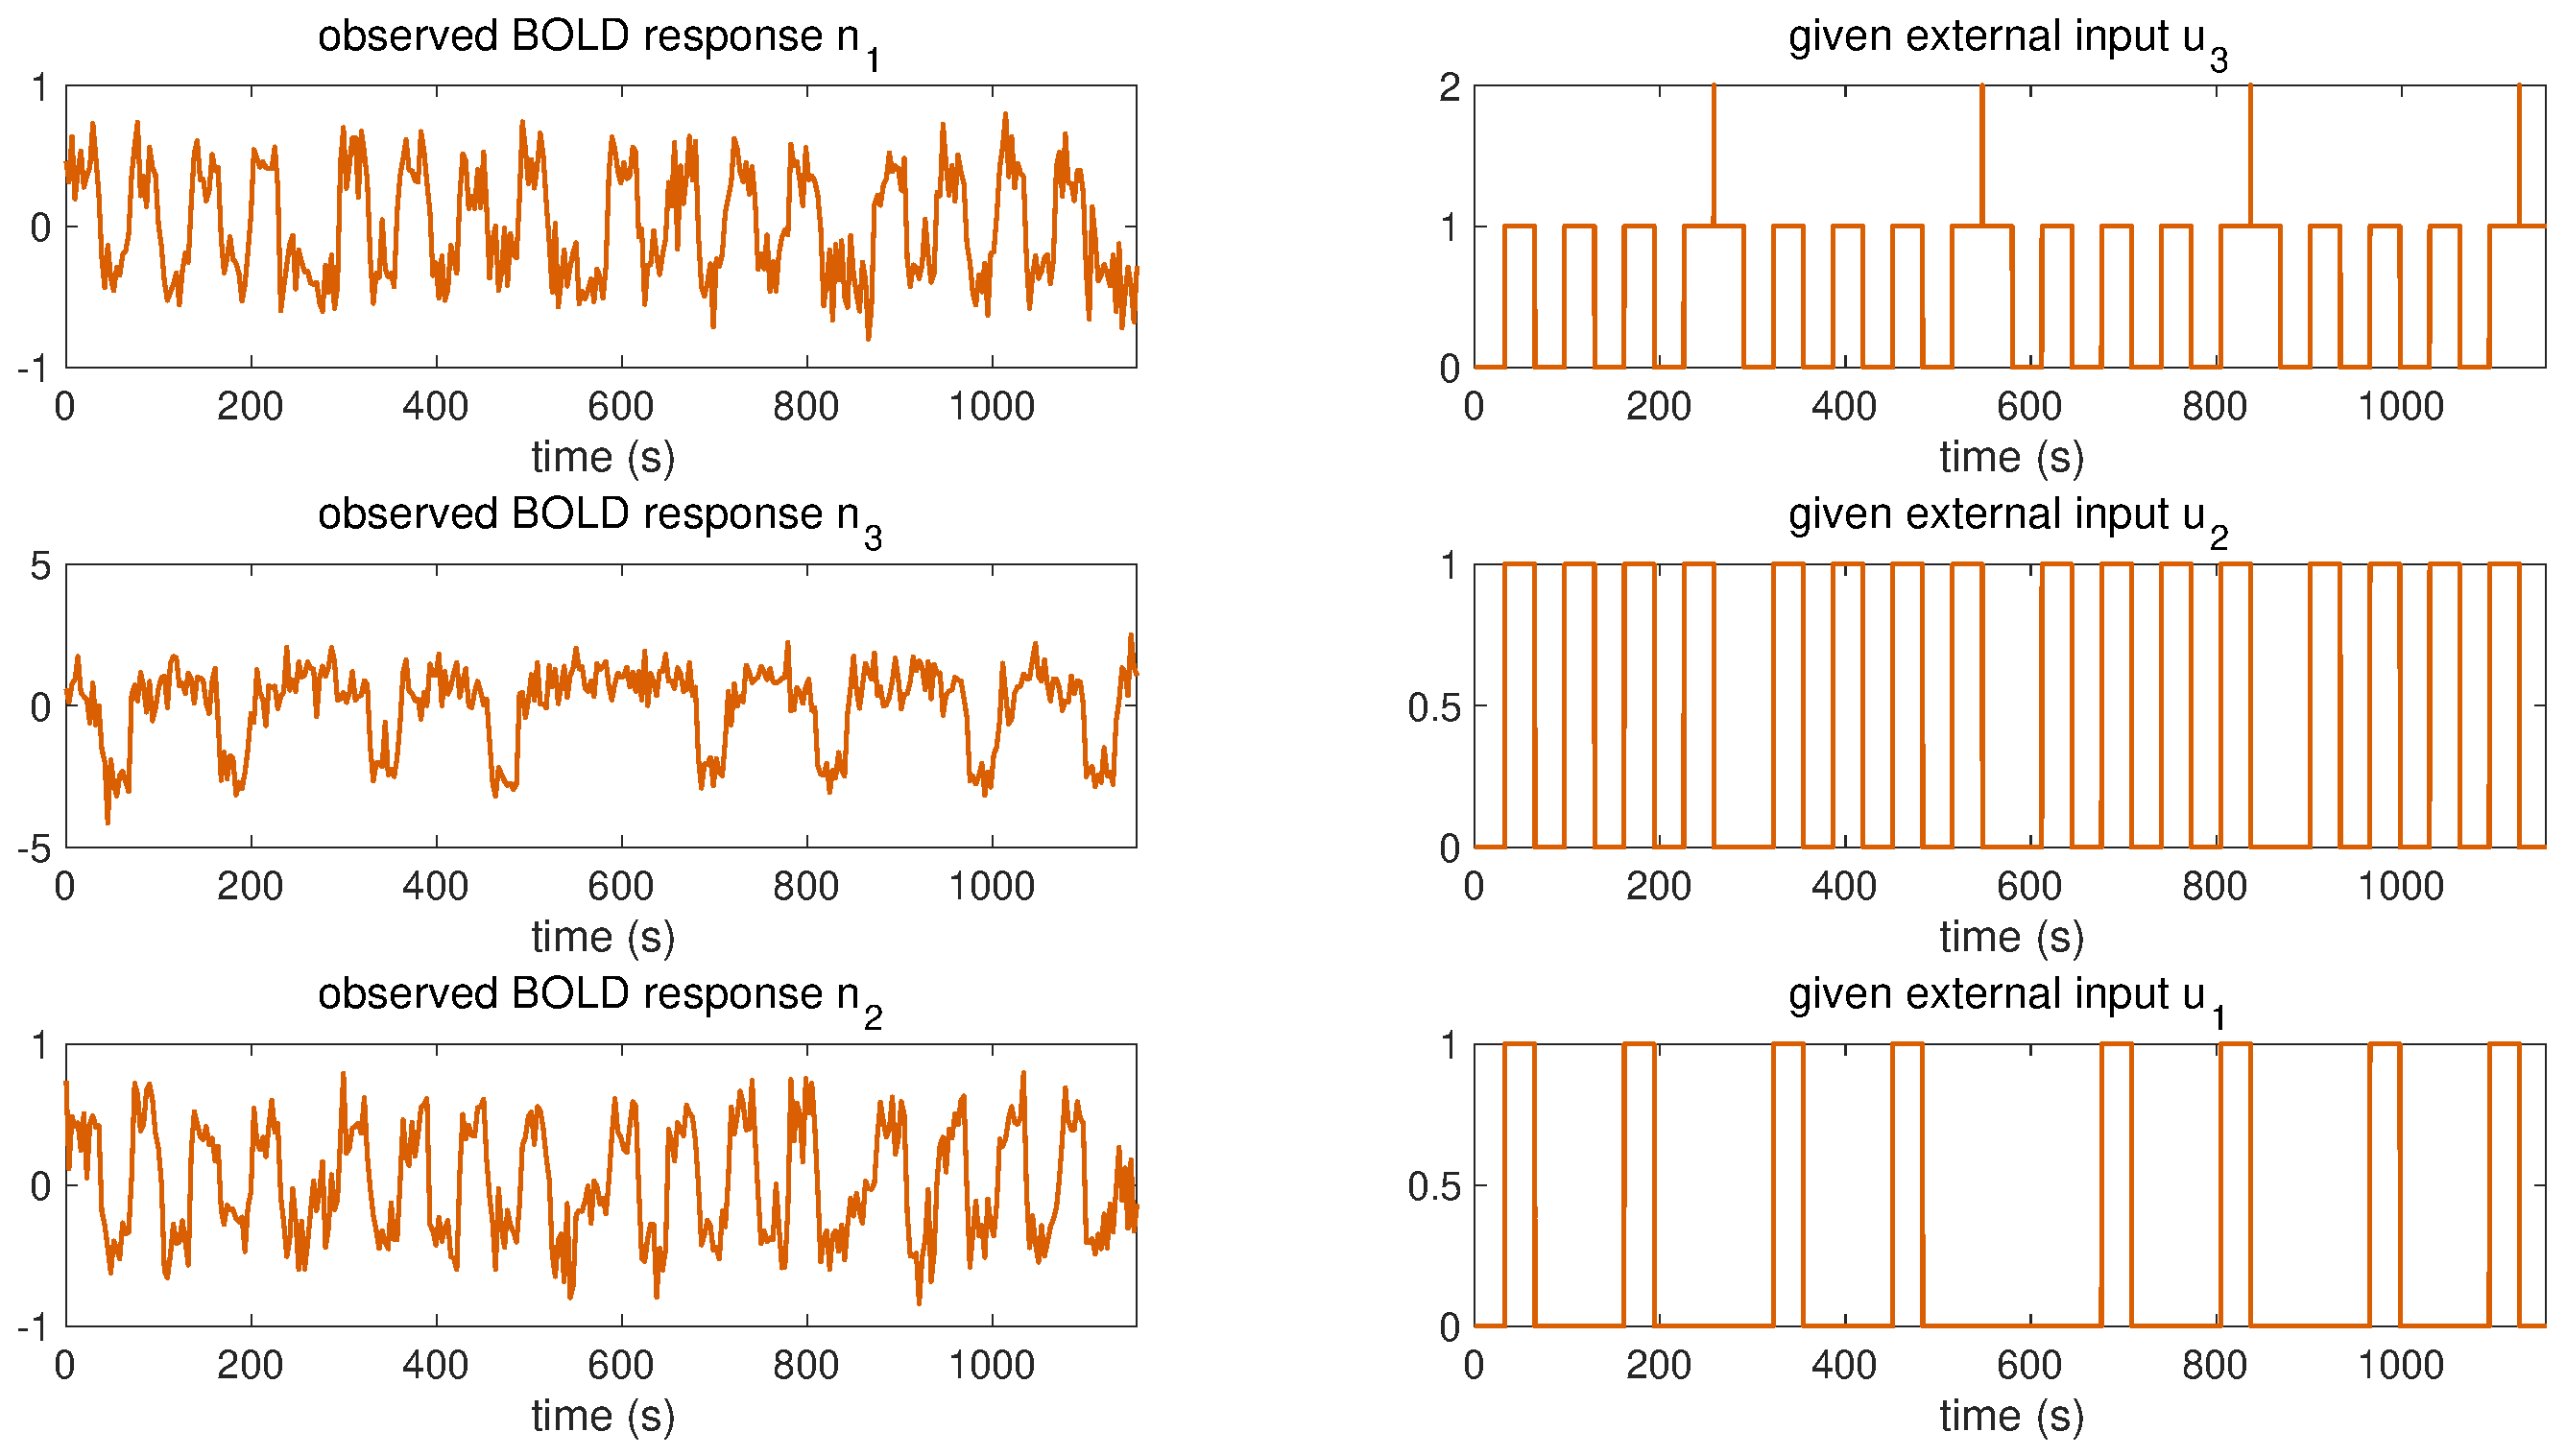
\includegraphics [width=4in]{VGM_for_dynamic_causal_modeling_01.eps}

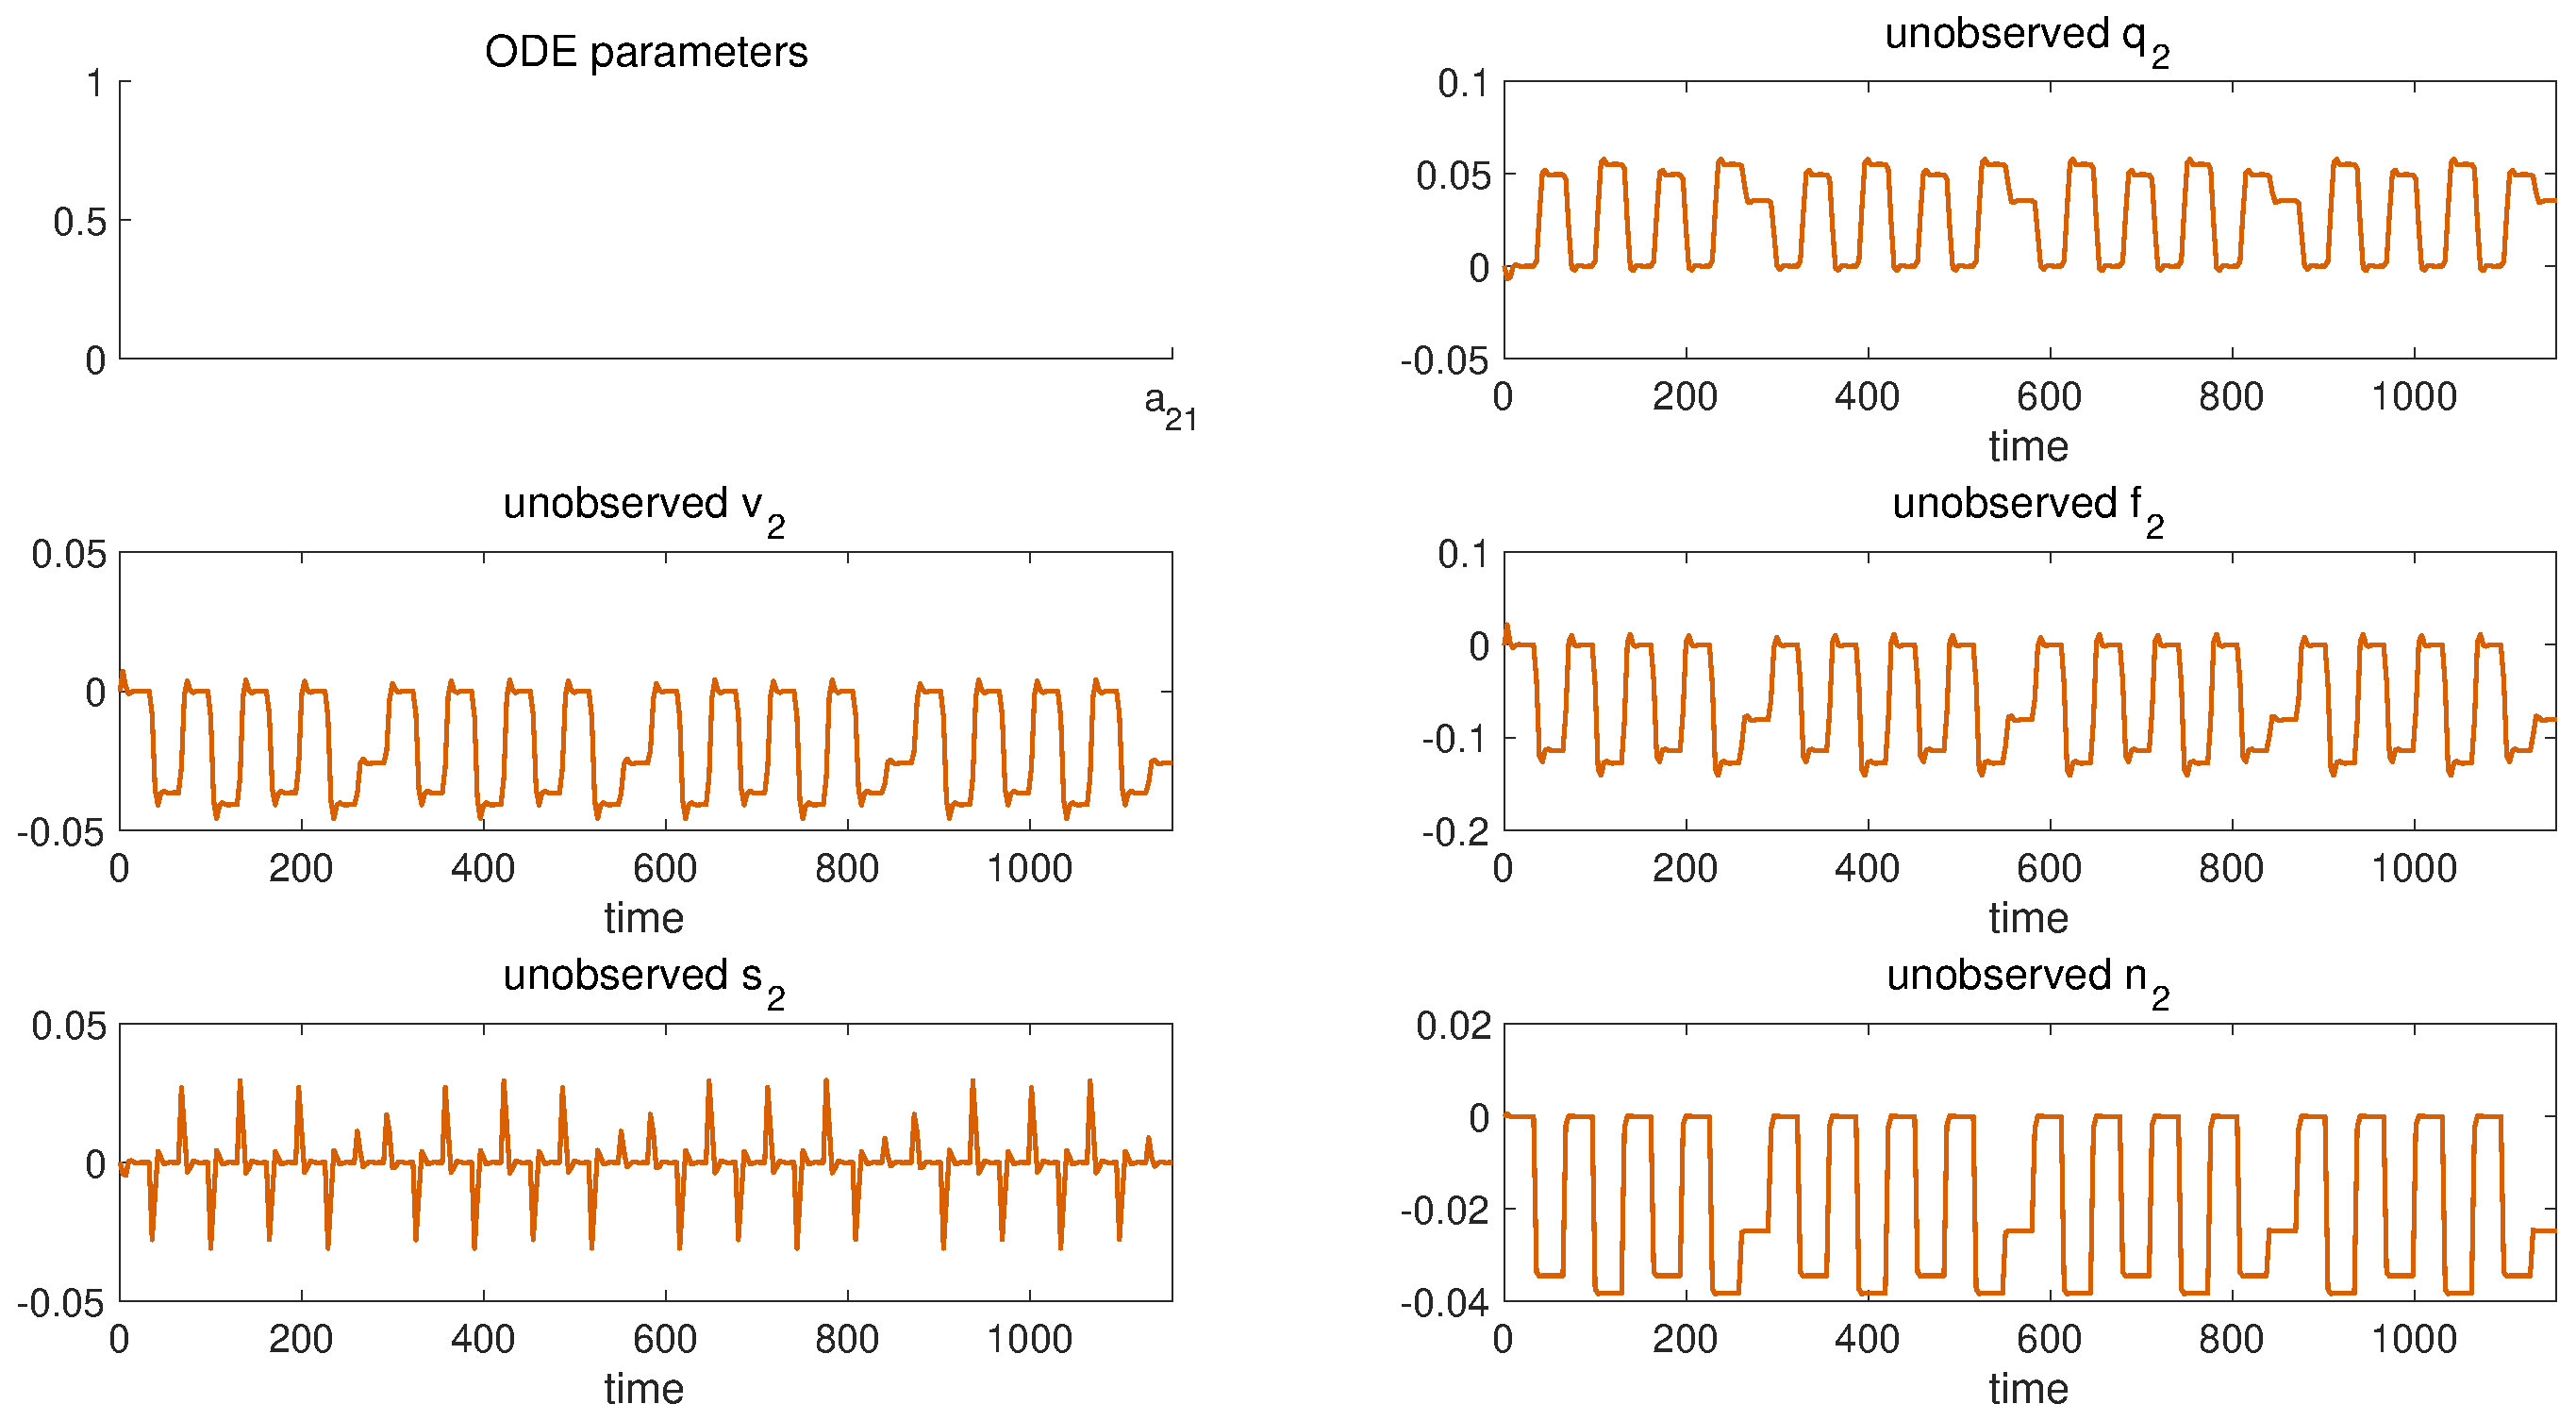
\includegraphics [width=4in]{VGM_for_dynamic_causal_modeling_02.eps}
\begin{verbatim}
end
\end{verbatim}


\subsection*{Mass Action Dynamical Systems}

\begin{par}
A deterministic dynamical system is represented by a set of $K$ ordinary differential equations (ODEs) with model parameters $\mathbf\theta \in \mathcal{R}^d$ that describe the evolution of $K$ states $\mathbf{x}(t) = [x_1(t),\ldots, x_K(t)]^T$ such that:
\end{par} \vspace{1em}
\begin{par}
$\dot{\mathbf{x}}(t) = \frac{d \mathbf{x}(t)}{d t} = \mathbf{f}(\mathbf{x}(t),\mathbf\theta) \qquad (1)$,
\end{par} \vspace{1em}
\begin{par}
A sequence of observations, $\mathbf{y}(t)$, is usually contaminated by measurement error which we assume to be normally distributed with zero mean and variance for each of the $K$ states, i.e. $\mathbf{E}\sim\mathcal{N}(\mathbf{E};\mathbf{0},\mathbf{D})$, with $\mathbf{D}_{ik}=\sigma_k ^2 \delta_{ik}$. For $N$ distinct time points the overall system may therefore be summarized as
\end{par} \vspace{1em}
\begin{par}
$\mathbf{Y} = \mathbf{X} + \mathbf{E}$,
\end{par} \vspace{1em}
\begin{par}
where
\end{par} \vspace{1em}
\begin{par}
$\mathbf{X} = [\mathbf{x}(t_1),\ldots,\mathbf{x}(t_N)] =  [\mathbf{x}_1,\ldots,\mathbf{x}_K]^T$,
\end{par} \vspace{1em}
\begin{par}
$\mathbf{Y} = [\mathbf{y}(t_1),\ldots,\mathbf{y}(t_N)] =  [\mathbf{y}_1,\ldots,\mathbf{y}_K]^T$,
\end{par} \vspace{1em}
\begin{par}
and $\mathbf{x}_k = [x_k(t_1),\ldots,x_k(t_N)]^T$ is the $k$'th state sequence and $\mathbf{y}_k = [y_k(t_1),\ldots,y_k(t_N)]^T$ are the observations. Given the observations $\mathbf{Y}$ and the description of the dynamical system (1), the aim is to estimate both state variables $\mathbf{X}$ and parameters $\mathbf\theta$.
\end{par} \vspace{1em}
\begin{par}
We consider only dynamical systems that are \_*locally linear \_*with respect to ODE parameters $\mathbf\theta$ and individual states $\mathbf{x}$. Such ODEs include mass-action kinetics and are given by:
\end{par} \vspace{1em}
\begin{par}
$f_{k}(\mathbf{x}(t),\theta) = \sum_{i=1} \theta_{ki} \prod_{j \in\mathcal{M}_{ki}} x_j \qquad (2)$,
\end{par} \vspace{1em}
\begin{par}
with \$\ensuremath{\backslash}mathcal\{M\}\_\{ki\} \ensuremath{\backslash}subseteq \ensuremath{\backslash}\{ 1, \ensuremath{\backslash}dots, K\ensuremath{\backslash}\}\$describing the state variables in each factor of the equation (i.e. the functions are linear in parameters and contain arbitrary large products of monomials of the states).
\end{par} \vspace{1em}
\begin{par}
start timer
\end{par} \vspace{1em}
\begin{verbatim}
tic;
\end{verbatim}


\subsection*{Prior on States and State Derivatives}

\begin{par}
Gradient matching with Gaussian processes assumes a joint Gaussian process prior on states and their derivatives:
\end{par} \vspace{1em}
\begin{par}
$\left(\begin{array}{c} \mathbf{X} \\ \dot{\mathbf{X}} \end{array}\right) \sim \mathcal{N} \left(\begin{array}{c} \mathbf{X} \\ \dot{\mathbf{X}} \end{array}~;~\begin{array}{c} \mathbf{0} \\\mathbf{0} \end{array}~,~\begin{array}{cc} \mathbf{C}_{\mathbf\phi} & \mathbf{C}_{\mathbf\phi}' \\ '\mathbf{C}_{\mathbf\phi} & \mathbf{C}_{\mathbf\phi}'' \end{array} \right) \qquad (3)$,
\end{par} \vspace{1em}
\begin{par}
with
\end{par} \vspace{1em}
\begin{par}
$\mathrm{cov}(x_k(t), x_k(t)) = C_{\mathbf\phi_k}(t,t')$,
\end{par} \vspace{1em}
\begin{par}
$\mathrm{cov}(\dot{x}_k(t), x_k(t)) = \frac{\partial C_{\mathbf{\phi}_k}(t,t')}{\partial t} =: C_{{\mathbf\phi}_k}'(t,t')$,
\end{par} \vspace{1em}
\begin{par}
$\mathrm{cov}(x_k(t), \dot{x}_k(t)) = \frac{\partial C_{\mathbf\phi_k}(t,t')}{\partial t'} =: {'C_{\mathbf\phi_k}(t,t')}$,
\end{par} \vspace{1em}
\begin{par}
$\mathrm{cov}(\dot{x}_k(t), \dot{x}_k(t)) = \frac{\partialC_{\mathbf\phi_k}(t,t') }{\partial t \partial t'} =: C_{\mathbf\phi_k}''(t,t')$.
\end{par} \vspace{1em}


\subsection*{Matching Gradients}

\begin{par}
Given the joint distribution over states and their derivatives (3) as well as the ODEs (2), we therefore have two expressions for the state derivatives:
\end{par} \vspace{1em}
\begin{par}
$\dot{\mathbf{X}} = \mathbf{F} + \mathbf\epsilon_1, \mathbf\epsilon_1 \sim\mathcal{N}\left(\mathbf\epsilon_1;\mathbf{0}, \mathbf{I}\gamma \right)$,
\end{par} \vspace{1em}
\begin{par}
$\dot{\mathbf{X}} = {'\mathbf{C}_{\mathbf\phi}} \mathbf{C}_{\mathbf\phi}^{-1}~\mathbf{X} + \mathbf\epsilon_2, \mathbf\epsilon_2 \sim\mathcal{N}\left(\mathbf\epsilon_2;\mathbf{0}, \mathbf{A} \right)$,
\end{par} \vspace{1em}
\begin{par}
where $\mathbf{F} := \mathbf{f}(\mathbf{X},\mathbf\theta)$ and $\mathbf{A} :=\mathbf{C}_{\mathbf\phi}'' -  {'\mathbf{C}_{\mathbf\phi}} \mathbf{C}_{\mathbf\phi}^{-1}\mathbf{C}_{\mathbf\phi}'$ and $\gamma$ is the error variance in the ODEs. Note that, in a deterministic system, the output of the ODEs $\mathbf{F}$ should equal the state derivatives $\dot{\mathbf{X}}$. However, in the first equation above we relax this contraint by adding stochasticity to the state derivatives $\dot{\mathbf{X}}$ in order to compensate for a
\end{par} \vspace{1em}
\begin{par}
potential model mismatch. The second equation above is obtained by deriving the conditional distribution for $\dot{\mathbf{X}}$ from the joint distribution in equation (3). Equating the two expressions in the equations above we can eliminate the unknown state derivatives $\dot{\mathbf{X}$:
\end{par} \vspace{1em}
\begin{par}
$\mathbf{F} = {'\mathbf{C}_{\mathbf\phi}} \mathbf{C}_{\mathbf\phi}^{-1} ~\mathbf{X} +\mathbf\epsilon_0 \qquad (4)$,
\end{par} \vspace{1em}
\begin{par}
with $\mathbf{\epsilon_0} := \mathbf{\epsilon_2} - \mathbf{\epsilon_1}$.
\end{par} \vspace{1em}
\begin{verbatim}
[dC_times_invC,inv_C,A_plus_gamma_inv] = kernel_function(kernel,state,time.est);
\end{verbatim}


\subsection*{Rewrite ODEs as Linear Combination in Parameters}

\begin{par}
Since, according to the mass action dynamics (equation 2), the ODEs are \textit{*linear in the parameters *}\$\ensuremath{\backslash}mathbf\ensuremath{\backslash}theta\$ we can rewrite the ODEs in equation (2) as a linear combination in the parameters:
\end{par} \vspace{1em}
\begin{par}
$\mathbf{B}_{\mathbf{\theta} k} \mathbf{\theta} + \mathbf{b}_{\mathbf{\theta} k} \stackrel{!}{=}\mathbf{f}_k(\mathbf{X},\mathbf{\theta}) \qquad (5)$,
\end{par} \vspace{1em}
\begin{par}
where matrices $\mathbf{B}_{\mathbf{\theta} k}$ and $\mathbf{b}_{\mathbf{\theta} k}$ and $\mathbf{b}_{\mathbf{\theta} k}$ are defined such that the ODEs $\mathbf{f}_k(\mathbf{X},\mathbf{\theta})$ are expressed as a linear combination in $\mathbf{\theta}$.
\end{par} \vspace{1em}
\begin{verbatim}
[ode_param.lin_comb.B,ode_param.lin_comb.b] = rewrite_odes_as_linear_combination_in_parameters(ode,symbols);
\end{verbatim}


\subsection*{Posterior over ODE Parameters}

\begin{par}
Inserting (5) into (4) and solving for $$\mathbf{\theta}$\$ yields:
\end{par} \vspace{1em}
\begin{par}
$\mathbf{\theta} = \mathbf{B}_{\mathbf{\theta}}^+ \left( {'\mathbf{C}_{\mathbf{\phi}}}\mathbf{C}_{\mathbf{\phi}}^{-1} \mathbf{X} - \mathbf{b}_{\mathbf{\theta}} + \mathbf{\epsilon_0}\right)$,
\end{par} \vspace{1em}
\begin{par}
where $\mathbf{B}_{\mathbf{\theta}}^+$ denotes the pseudo-inverse of $\mathbf{B}_{\mathbf{\theta}}$. Since $$\mathbf{C}_{\mathbf{\phi}}$\$ is block diagonal we can rewrite the expression above as:
\end{par} \vspace{1em}
\begin{par}
$\mathbf{\theta} = \left( \mathbf{B}_{\mathbf{\theta}}^T \mathbf{B}_{\mathbf{\theta}} \right)^{-1} ~\mathbf{B}_{\mathbf{\theta}}^T  \left( \sum_k {'\mathbf{C}_{\mathbf{\phi}_k}}\mathbf{C}_{\mathbf{\phi}_k}^{-1} \mathbf{X}_k - \mathbf{b}_{\mathbf{\theta} k} + \mathbf{\epsilon_0}^{(k)} \right)\\ ~= \left( \mathbf{B}_{\mathbf{\theta}}^T \mathbf{B}_{\mathbf{\theta}} \right)^{-1} \left(\sum_k \mathbf{B}_{\mathbf{\theta} k}^T \left( {'\mathbf{C}_{\mathbf{\phi}_k}}\mathbf{C}_{\mathbf{\phi}_k}^{-1} \mathbf{X}_k - \mathbf{b}_{\mathbf{\theta} k} +\mathbf{\epsilon_0}^{(k)} \right) \right)$,
\end{par} \vspace{1em}
\begin{par}
where we subsitute the Moore-Penrose inverse for the pseudo-inverse (i.e. $\mathbf{B}_{\mathbf{\theta}}^+ := \left( \mathbf{B}_{\mathbf{\theta}}^T \mathbf{B}_{\mathbf{\theta}}\right)^{-1} \mathbf{B}_{\mathbf{\theta}}^T$). We can therefore derive the posterior distribution over ODE parameters:
\end{par} \vspace{1em}
\begin{par}
$p(\mathbf{\theta} \mid \mathbf{X}, \mathbf{\phi}, \gamma) = \mathcal{N}\left(\mathbf{\theta} ; \left( \mathbf{B}_{\mathbf{\theta}}^T\mathbf{B}_{\mathbf{\theta}} \right)^{-1} \left( \sum_k \mathbf{B}_{\mathbf{\theta} k}^T ~\left( {'\mathbf{C}_{\mathbf{\phi} k}} \mathbf{C}_{\mathbf{\phi} k}^{-1} \mathbf{X}_k -\mathbf{b}_{\mathbf{\theta} k} \right) \right), ~ \mathbf{B}_{\mathbf{\theta}}^+ ~(\mathbf{A} + \mathbf{I}\gamma) ~ \mathbf{B}_{\mathbf{\theta}}^{+T} \qquad (6)$.
\end{par} \vspace{1em}


\subsection*{Rewrite Hemodynamic ODEs as Linear Combination in (monotonic functions of) Individual Hemodynamic States}

\begin{itemize}
\setlength{\itemsep}{-1ex}
   \item *Deoxyhemoglobin content *
\end{itemize}

\begin{verbatim}               Rewrite the BOLD signal change equation as a linear combination
in a monotonic function of the deoxyhemoglobin content $$\exp(\mathbf{q})$$:\end{verbatim}
    
\begin{verbatim}               $$\mathbf{R}_{q~\mathbf\lambda} ~ \exp(\mathbf{q}) ~+ ~
\mathbf{r}_{v~\mathbf\lambda} \stackrel{!}{=} ~\mathbf\lambda(\mathbf{q},\mathbf{v})$$.\end{verbatim}
    \begin{verbatim}
         [state.deoxyhemo.R,state.deoxyhemo.r] = rewrite_bold_signal_eqn_as_linear_combination_in_deoxyhemo(symbols);
\end{verbatim}
\begin{par}

\end{par} \vspace{1em}
\begin{itemize}
\setlength{\itemsep}{-1ex}
   \item \textbf{Blood volume}
\end{itemize}

\begin{verbatim}               Rewrite the deoxyhemoglobin content ODE as a linear combination
in a monotonic function of the blood volume $\exp\left( 17 / 8 ~\mathbf{v}\right)$:\end{verbatim}
    
\begin{verbatim}                $\mathbf{R}_{v\dot{q}} ~\exp\left( 17 / 8 ~\mathbf{v}\right)
~+~ \mathbf{r}_{v\dot{q}} \stackrel{!}{=} \mathbf{f}_{\dot{q}}(\mathbf{X},\mathbf\theta)$.\end{verbatim}
    \begin{verbatim}
         [state.vol.R,state.vol.r] = rewrite_deoxyhemo_ODE_as_linear_combination_in_vol(ode,symbols);
\end{verbatim}
\begin{par}

\end{par} \vspace{1em}
\begin{itemize}
\setlength{\itemsep}{-1ex}
   \item \textbf{Blood flow}
\end{itemize}

\begin{verbatim}               Rewrite the blood volume ODE as a linear combination in
a monotonic function of the blood flow $\exp(\mathbf{f})$:\end{verbatim}
    
\begin{verbatim}                  $$\mathbf{R}_{f~\dot{v}} ~ \exp(\mathbf{f}) + \mathbf{r}_{f~\dot{v}}
\stackrel{!}{=} \mathbf{f}_{\dot{v}}(\mathbf{X},\mathbf\theta)$$.\end{verbatim}
    \begin{verbatim}
         [state.flow.R,state.flow.r] = rewrite_vol_ODE_as_linear_combination_in_flow(ode,symbols);
\end{verbatim}
\begin{itemize}
\setlength{\itemsep}{-1ex}
   \item \textbf{Vasosignalling}
\end{itemize}

\begin{verbatim}               Rewrite the blood flow and vasoginalling ODEs as a linear
combination in vasosignalling $\mathbf{s}$:\end{verbatim}
    
\begin{verbatim}                   $$\mathbf{R}_{s\dot{f}} ~\mathbf{s} + \mathbf{r}_{s\dot{f}}
\stackrel{!}{=} \mathbf{f}_{\dot{f}}(\mathbf{X},\mathbf\theta)$$.\end{verbatim}
    
\begin{verbatim}                   $$\mathbf{R}_{s\dot{s}}~ \mathbf{s} + \mathbf{r}_{s\dot{s}}
\stackrel{!}{=} \mathbf{f}_{\dot{s}}(\mathbf{X},\mathbf\theta)$$.\end{verbatim}
    \begin{verbatim}
        [state.vaso.R,state.vaso.r] = rewrite_vaso_and_flow_odes_as_linear_combination_in_vaso(ode,symbols);
\end{verbatim}


\subsection*{Rewrite Neuronal ODEs as Linear Combination in Individual Neuronal States}

\begin{par}
We rewrite the ODE(s) $$\mathbf{f}_k(\mathbf{X},\mathbf\theta)$\$ as a linear combination in the individual state $$\mathbf{n}_u$\$:
\end{par} \vspace{1em}

\begin{verbatim}       $$\mathbf{R}_{uk}  \mathbf{n}_u + \mathbf{r}_{uk} \stackrel{!}{=}
\mathbf{f}_{k}(\mathbf{X},\mathbf\theta)$$,\end{verbatim}
    \begin{par}
where matrices $$\mathbf{R}_{uk}$\$ and $\mathbf{r}_{uk}$ are defined such that the ODE $$\mathbf{f}_k(\mathbf{X},\mathbf\theta)$\$ is expressed as a linear combination in the individual state $$\mathbf{n}_u$\$.
\end{par} \vspace{1em}
\begin{verbatim}
[state.neuronal.R,state.neuronal.r] = rewrite_odes_as_linear_combination_in_ind_neuronal_states(ode,symbols,coupling_idx.states);
\end{verbatim}


\subsection*{Posterior over Individual States}

\begin{par}
Given the linear combination of the ODEs w.r.t. an individual state, we define the matrices $\mathbf{B}_u$ and $\mathbf{b}_u$ such that the expression $$\mathbf{f}(\mathbf{X},\mathbf{\theta}) - {'\mathbf{C}}_{\mathbf{\phi}}\mathbf{C}_{\mathbf{\phi}}^{-1} \mathbf{X}$\$ is rewritten as a linear combination in an individual state $\mathbf{x}_u$:
\end{par} \vspace{1em}
\begin{par}
$\mathbf{B}_{u} \mathbf{x}_u + \mathbf{b}_{u} \stackrel{!}{=}\mathbf{f}(\mathbf{X},\mathbf{\theta}) - {'\mathbf{C}}_{\mathbf{\phi}}\mathbf{C}_{\mathbf{\phi}}^{-1} \mathbf{X} \qquad (7)$.
\end{par} \vspace{1em}
\begin{par}
Inserting (7) into (4) and solving for $$\mathbf{x}_u$\$ yields:
\end{par} \vspace{1em}
\begin{par}
$$\mathbf{x}_u = \mathbf{B}_{u}^+ \left( \mathbf{\epsilon_0} -\mathbf{b}_{u}\right)$\$,
\end{par} \vspace{1em}
\begin{par}
where $$\mathbf{B}_{u}^+$\$ denotes the pseudo-inverse of $$\mathbf{B}_{u}$\$. Since $$\mathbf{C}_{\mathbf{\phi}}$\$ is block diagonal we can rewrite the expression above as:
\end{par} \vspace{1em}
\begin{par}
$\mathbf{x}_u = \left( \mathbf{B}_{u} \mathbf{B}_{u}^T \right)^{-1}\mathbf{B}_{u}^T \sum_k \left(\mathbf{\epsilon_0}^{(k)} -\mathbf{b}_{uk} \right)\\ \quad= \left( \mathbf{B}_{u} \mathbf{B}_{u}^T \right)^{-1} \sum_k\mathbf{B}_{uk}^T \left(\mathbf{\epsilon_0}^{(k)} -\mathbf{b}_{uk} \right)$,
\end{par} \vspace{1em}
\begin{par}
where we subsitute the Moore-Penrose inverse for the pseudo-inverse (i.e. $\mathbf{B}_{\mathbf{\theta}}^+ := \left( \mathbf{B}_{\mathbf{\theta}}^T \mathbf{B}_{\mathbf{\theta}}\right)^{-1} \mathbf{B}_{\mathbf{\theta}}^T$).  We can therefore derive the posterior distribution over an individual state $$\mathbf{x}_{u}$\$:
\end{par} \vspace{1em}
\begin{par}
$p(\mathbf{x}_u \mid \mathbf{X}_{-u}, \mathbf{\phi}, \gamma)= \mathcal{N}\left(\mathbf{x}_u ; \left( \mathbf{B}_{u} \mathbf{B}_{u}^T\right)^{-1} \left( - \sum_k \mathbf{B}_{uk}^T \mathbf{b}_{uk} \right),~\mathbf{B}_{u}^{+} ~ (\mathbf{A} + \mathbf{I}\gamma) ~ \mathbf{B}_u^{+T}\right) \qquad (8)$,
\end{par} \vspace{1em}
\begin{par}
with $$\mathbf{X}_{-u}$\$ denoting the set of all states except state $$\mathbf{x}_u$\$.
\end{par} \vspace{1em}


\subsection*{Mean-field Variational Inference}

\begin{par}
To infer the parameters $$\mathbf{\theta}$\$, we want to find the maximum a posteriori estimate (MAP):
\end{par} \vspace{1em}
\begin{par}
$\mathbf{\theta}^* := \mathrm{arg} \max_{\mathbf{\theta}} ~ \ln p(\mathbf{\theta} \mid\mathbf{Y},\mathbf{\phi},\gamma,\mathbf \sigma)\\ \quad= \mathrm{arg}\max_{\mathbf{\theta}} ~ \ln \int  p(\mathbf{\theta},\mathbf{X} \mid\mathbf{Y},\mathbf{\phi},\gamma,\mathbf\sigma) d\mathbf{X}\\ \quad= \mathrm{arg}\max_{\mathbf{\theta}} ~ \ln \int p(\mathbf{\theta} \mid \mathbf{X},\mathbf{\phi},\gamma)p(\mathbf{X} \mid \mathbf{Y}, \mathbf{\phi},\mathbf\sigma) d\mathbf{X} \qquad(9)$.
\end{par} \vspace{1em}
\begin{par}
However, the integral above is intractable due to the strong couplings induced by the nonlinear ODEs $$\mathbf{f}$\$ which appear in the term $$p(\mathbf{\theta} \mid \mathbf{X},\mathbf{\phi},\gamma)$\$.
\end{par} \vspace{1em}
\begin{par}
We use mean-field variational inference to establish variational lower bounds that are analytically tractable by decoupling state variables from the ODE parameters as well as decoupling the state variables from each other. Note that, since the ODEs described by equation (2) are \textit{*locally linear}*, both conditional distributions $$p(\mathbf{\theta} \mid\mathbf{X},\mathbf{Y},\mathbf{\phi},\gamma,\mathbf\sigma)$\$ (equation (6)) and $$p(\mathbf{x}_u \mid \mathbf{\theta},\mathbf{X}_{-u},\mathbf{Y},\mathbf{\phi},\gamma,\mathbf\sigma)$\$ (equation (8)) are analytically tractable and Gaussian distributed as mentioned previously. The decoupling is induced by designing a variational distribution $$Q(\mathbf{\theta},\mathbf{X})$\$ which is restricted to the family of factorial distributions:
\end{par} \vspace{1em}
\begin{par}
$$\mathcal{Q} := \bigg{\{} Q : Q(\mathbf{\theta},\mathbf{X}) = q(\mathbf{\theta}) \prod_uq(\mathbf{x}_u) \bigg{\}}$\$.
\end{par} \vspace{1em}
\begin{par}
The particular form of $$q(\mathbf{\theta})$\$ and $$q(\mathbf{x}_u)$\$ are designed to be Gaussian distributed which places them in the same family as the true full conditional distributions. To find the optimal factorial distribution we minimize the Kullback-Leibler divergence between the variational and the true posterior distribution:
\end{par} \vspace{1em}
\begin{par}
$$\hat{Q} := \mathrm{arg} \min_{Q(\mathbf{\theta},\mathbf{X}) \in \mathcal{Q}} \mathrm{KL}\left[ Q(\mathbf{\theta},\mathbf{X}) \mid \mid p(\mathbf{\theta},\mathbf{X} \mid\mathbf{Y},\mathbf{\phi}, \gamma,\mathbf\mathbf{\sigma}) \right] \qquad (10)$\$,
\end{par} \vspace{1em}
\begin{par}
where $$\hat{Q}$\$ is the proxy distribution. The proxy distribution that minimizes the KL-divergence (10) depends on the true full conditionals and is given by:
\end{par} \vspace{1em}
\begin{par}
$\hat{q}({\mathbf{\theta}}) \propto \exp \left(~ E_{Q_{-\mathbf{\theta}}} \ln p(\mathbf{\theta} \mid\mathbf{X},\mathbf{Y},\mathbf{\phi},\gamma,\mathbf\mathbf{\sigma}) ~\right) \qquad (11)\\\hat{q}(\mathbf{x}_u) \propto \exp\left( ~ E_{Q_{-u}} \ln p(\mathbf{x}_u\mid \mathbf{\theta}, \mathbf{X}_{-u},\mathbf{Y},\mathbf{\phi},\gamma,\mathbf{\sigma}) ~ \right)\qquad (12)$.
\end{par} \vspace{1em}


\subsection*{Denoising BOLD Observations}

\begin{par}
We denoise the BOLD observation by standard GP regression.
\end{par} \vspace{1em}
\begin{verbatim}
bold_response.denoised_obs = denoising_BOLD_observations(simulation.bold_response{:,{'n_1','n_3','n_2'}},inv_C,symbols,simulation);
\end{verbatim}


\subsection*{Fitting observations of state trajectories}

\begin{par}
We fit the observations of state trajectories by standard GP regression. The data-informed distribution\$ $p(\mathbf{X} \mid \mathbf{Y}, \mathbf{\phi},\mathbf\mathbf{\sigma})$\$ in euqation (9) can be determined analytically using Gaussian process regression with the GP prior $$p(\mathbf{X} \mid\mathbf{\phi}) = \prod_k \mathcal{N}(\mathbf{x}_k ;\mathbf{0},\mathbf{C}_{\mathbf{\phi}_k})$\$:
\end{par} \vspace{1em}
\begin{par}
$$p(\mathbf{X} \mid \mathbf{Y}, \mathbf{\phi},\gamma) = \prod_k\mathcal{N}(\mathbf{x}_k ;\mathbf\mu_k(\mathbf{y}_k),\mathbf\mathbf{\sigma}_k)$\$,
\end{par} \vspace{1em}
\begin{par}
where $$\mathbf\mu_k(\mathbf{y}_k) := \mathbf{\sigma}_k^{-2} \left(\mathbf{\sigma}_k^{-2}\mathbf{I} + \mathbf{C}_{\mathbf{\phi}_k}^{-1} \right)^{-1} \mathbf{y}_k$\$ and $$\mathbf{\sigma}_k ^{-1}:=\mathbf{\sigma}_k^{-2} \mathbf{I} +\mathbf{C}_{\mathbf\mathbf{\phi}_k}^{-1}$\$.
\end{par} \vspace{1em}
\begin{verbatim}
[mu,inv_sigma] = fitting_state_observations(inv_C,obs_to_state_relation,simulation,symbols);
\end{verbatim}


\subsection*{Coordinate Ascent Variational Gradient Matching}

\begin{par}
We minimize the KL-divergence in equation (10) by coordinate descent (where each step is analytically tractable) by iterating between determining the proxy for the distribution over ODE parameters $$\hat{q}(\mathbf{\theta})$\$ and the proxies for the distribution over individual states $$\hat{q}(\mathbf{x}_u)$\$.
\end{par} \vspace{1em}
\begin{itemize}
\setlength{\itemsep}{-1ex}
   \item \textbf{Initialize the state estimation by the GP regression posterior}
\end{itemize}
\begin{par}

\end{par} \vspace{1em}
\begin{verbatim}
state.proxy.mean = array2table([time.est',mu],'VariableNames',['time',symbols.state_string]);
bold_response.obs_old = bold_response.denoised_obs;
ode_param.proxy.mean = zeros(length(symbols.param),1);
\end{verbatim}
\begin{par}

\end{par} \vspace{1em}
\begin{itemize}
\setlength{\itemsep}{-1ex}
   \item \textbf{Coordinate ascent}
\end{itemize}
\begin{par}

\end{par} \vspace{1em}
\begin{verbatim}
            for i = 1:opt_settings.coord_ascent_numb_iter
\end{verbatim}


\subsection*{Proxy for Hemodynamic States}

\begin{par}
Determine the proxies for the states, starting with deoxyhemoglobin followed by blood volume, blood flow and finally vasosignalling. The information flow in the hemodynamic system is shown in its factor graph below:
\end{par} \vspace{1em}
\begin{par}
.
\end{par} \vspace{1em}
\begin{par}
The model inversion in the hemodynmic factor graph above occurs locally w.r.t. individual states. Given the expression for the BOLD signal change equation, we invert the BOLD signal change equation analytically to determine the deoxyhemoglobin content $$\mathbf{q}$\$ (1). The newly inferred deoxyhemoglobin content $$\mathbf{q}$\$ influences the expression for the factor associated with the change in deoxyhemoglobin content $$\mathbf{h}_{\dot{\mathbf{q}}}$\$, which we subsequently invert analytically to infer the blood volume $\mathbf{v}$ (2). Thereafter, we infer the blood flow $$\mathbf{f}$\$ (3) by inverting the factors associated with the change in blood volume $$\mathbf{h}_{\dot{\mathbf{v}}}$\$ as well as vasosignalling $$\mathbf{h}_{\dot{\mathbf{s}}}$\$, followed by inferring vasosignalling $$\mathbf{s}$\$ (4) by inverting the factors associated with blood flow induction $$\mathbf{h}_{\dot{\mathbf{f}}}$\$ and vasosignalling $$\mathbf{h}_{\dot{\mathbf{s}}}$\$. Finally, the neuronal dynamics (5) are learned, in part, by inverting the factor associated with vasosignalling $$\mathbf{h}_{\dot{\mathbf{s}}}$\$. The typical trajectories of each of the states are shown (red) together with their iterative approximation (grey lines) obtained by graphical DCM.
\end{par} \vspace{1em}
\begin{itemize}
\setlength{\itemsep}{-1ex}
   \item \textbf{Proxy for deoxyhemolgobin content}
\end{itemize}

\begin{verbatim}               Damping is required since we invert only the factor for
the BOLD signal change equation w.r.t. a monotonic function of deoxyhemoglobin
content $\exp( \mathbf{q})$.\end{verbatim}
    
\begin{verbatim}                          * Undamped proxy:*\end{verbatim}
    \begin{par}

\end{par} \vspace{1em}
\begin{verbatim}
                state_proxy_undamped = proxy_for_deoxyhemoglobin_content(state.deoxyhemo,state.proxy.mean{:,symbols.state_string},...
                    bold_response.denoised_obs,symbols,A_plus_gamma_inv,opt_settings);
\end{verbatim}

\begin{verbatim}                          * *\end{verbatim}
    \begin{itemize}
\setlength{\itemsep}{-1ex}
   \item Damped proxy:*
\end{itemize}
\begin{par}

\end{par} \vspace{1em}
\begin{verbatim}
                state.proxy.mean{:,{'q_1','q_3','q_2'}} = (1-opt_settings.damping) * state.proxy.mean{:,{'q_1','q_3','q_2'}} + ...
                    opt_settings.damping * state_proxy_undamped;
\end{verbatim}
\begin{itemize}
\setlength{\itemsep}{-1ex}
   \item \textbf{Proxy for blood volume}
\end{itemize}
\begin{itemize}
\setlength{\itemsep}{-1ex}
   \item *    Damping is required since we invert only the a subset of ODEs w.r.t. a monotonic function of blood volume $\exp\left( 17/ 8 ~ \mathbf{v} \right)$.
\end{itemize}
\begin{itemize}
\setlength{\itemsep}{-1ex}
   \item *
\end{itemize}
\begin{itemize}
\setlength{\itemsep}{-1ex}
   \item Undamped proxy:*
\end{itemize}
\begin{par}

\end{par} \vspace{1em}
\begin{verbatim}
                state_proxy_undamped = proxy_for_blood_volume(state.vol,dC_times_invC,state.proxy.mean{:,symbols.state_string},...
                    ode_param.proxy.mean,symbols,A_plus_gamma_inv,opt_settings);
\end{verbatim}
\begin{itemize}
\setlength{\itemsep}{-1ex}
   \item Damped proxy:*
\end{itemize}
\begin{par}

\end{par} \vspace{1em}
\begin{verbatim}
                state.proxy.mean{:,{'v_1','v_3','v_2'}} = (1-opt_settings.damping) * state.proxy.mean{:,{'v_1','v_3','v_2'}} + ...
                    opt_settings.damping * state_proxy_undamped;
\end{verbatim}
\begin{itemize}
\setlength{\itemsep}{-1ex}
   \item \textbf{Proxy for blood flow}
\end{itemize}

\begin{verbatim}               Damping is required since we invert only the a subset of
ODEs w.r.t. a mononic function of blood flow $\exp(\mathbf{f})$.\end{verbatim}
    \begin{itemize}
\setlength{\itemsep}{-1ex}
   \item Undamped proxy:*
\end{itemize}
\begin{par}

\end{par} \vspace{1em}
\begin{verbatim}
                state_proxy_undamped = proxy_for_blood_flow(state.flow,dC_times_invC,state.proxy.mean{:,symbols.state_string},...
                    ode_param.proxy.mean,symbols,A_plus_gamma_inv,opt_settings);
\end{verbatim}
\begin{itemize}
\setlength{\itemsep}{-1ex}
   \item Damped proxy:*
\end{itemize}
\begin{par}

\end{par} \vspace{1em}
\begin{verbatim}
                state.proxy.mean{:,{'f_1','f_3','f_2'}} = (1-opt_settings.damping) * state.proxy.mean{:,{'f_1','f_3','f_2'}} + ...
                    opt_settings.damping * state_proxy_undamped;
\end{verbatim}
\begin{par}

\end{par} \vspace{1em}
\begin{itemize}
\setlength{\itemsep}{-1ex}
   \item \textbf{Proxy for vasosignalling}
\end{itemize}

\begin{verbatim}               No damping is required because we invert all ODEs w.r.t.
vasosingalling $\mathbf{s}$.\end{verbatim}
    \begin{verbatim}
                state.proxy.mean{:,{'s_1','s_3','s_2'}} = proxy_for_vasosignalling(state.vaso,dC_times_invC,...
                    state.proxy.mean{:,symbols.state_string},ode_param.proxy.mean,symbols,A_plus_gamma_inv,opt_settings);
\end{verbatim}


\subsection*{Proxy for Neuronal States}

\begin{itemize}
\setlength{\itemsep}{-1ex}
   \item *Determine the proxies for the neuronal states. An example of the information flow in the neuronal part of the nonlinear forward modulating (nonlin\_fwd\_mod) is shown in its factor graph below:
\end{itemize}
\begin{par}
.
\end{par} \vspace{1em}

\begin{verbatim}                          In the neuronal factor graph (for the nonlinear
forwad modulation) above each individual state appears linear in every factor
in the neuronal model. We can therefore analytically invert every factor to
determine the neuronal state. The typical trajectories of each of the states
are shown (red) together with their iterative approximation (grey lines) obtained
by variational gradient matching.\end{verbatim}
    \begin{par}
No damping is required because we invert all ODEs w.r.t. neuronal populations $\mathbf{n}$.
\end{par} \vspace{1em}
\begin{verbatim}
                state.proxy.mean{:,{'n_1','n_3','n_2'}} = proxy_for_neuronal_populations(state.neuronal,...
                    state.proxy.mean{:,symbols.state_string},ode_param.proxy.mean',dC_times_invC,...
                    coupling_idx.states,symbols,A_plus_gamma_inv,opt_settings);
\end{verbatim}
\begin{par}

\end{par} \vspace{1em}
\begin{par}

\end{par} \vspace{1em}
\begin{par}
Keep initial value at zero:
\end{par} \vspace{1em}
\begin{par}

\end{par} \vspace{1em}
\begin{verbatim}
                state_idx = cellfun(@(x) ~strcmp(x(1),'u'),symbols.state_string);
                state.proxy.mean{:,symbols.state_string(state_idx)} = bsxfun(@minus,state.proxy.mean{:,symbols.state_string(state_idx)},...
                    state.proxy.mean{1,symbols.state_string(state_idx)});
\end{verbatim}


\subsection*{*            *}



\subsection*{}



\subsection*{\textbf{Proxy for ODE parameters}}

\begin{par}

\end{par} \vspace{1em}

\begin{verbatim}                   Expanding the proxy distribution in equation (11) for
$$\mathbf{\theta}$$ yields:\end{verbatim}
    
\begin{verbatim}                          $\hat{q}(\mathbf{\mathbf\theta}) \propto \exp
\left( ~E_{Q_{-\mathbf\theta}}     \ln p(\theta \mid \mathbf{X},\mathbf{Y},\mathbf\phi,\gamma,\mathbf\sigma)
~     \right) \\ \qquad= \exp \left( ~E_{Q_{-\mathbf{\theta}}} \ln \mathcal{N}\left(\mathbf{\theta}
; \left(    \mathbf{B}_{\mathbf{\theta}}^T \mathbf{B}_{\mathbf{\theta}} \right)^{-1}
\left( \sum_k    \mathbf{B}_{\mathbf{\theta} k}^T ~ \left( {'\mathbf{C}_{\mathbf{\phi}
k}}    \mathbf{C}_{\mathbf{\phi} k}^{-1} \mathbf{X}_k - \mathbf{b}_{\mathbf{\theta}
k} \right)    \right), ~ \mathbf{B}_{\mathbf{\theta}}^+ ~ (\mathbf{A} + \mathbf{I}\gamma)
~    \mathbf{B}_{\mathbf{\theta}}^{+T} \right) ~\right)$,\end{verbatim}
    
\begin{verbatim}                   where we substitute $$p(\mathbf{\theta} \mid \mathbf{X},\mathbf{\phi},\gamma)$$
with its density given in equation (6).\end{verbatim}
    
\begin{verbatim}                   No damping is required because we invert all ODEs w.r.t.
neuronal couplings $\mathbf{\theta}$.\end{verbatim}
    \begin{verbatim}
            if i>200 || i==opt_settings.coord_ascent_numb_iter
                [ode_param.proxy.mean,ode_param.proxy.inv_cov] = proxy_for_ode_parameters(...
                    state.proxy.mean{:,symbols.state_string},dC_times_invC,ode_param.lin_comb,...
                    symbols,A_plus_gamma_inv,opt_settings);
            end
\end{verbatim}


\subsection*{}



\subsection*{*            *}



\subsection*{\textbf{Intercept due to Confounding Effects}}


\begin{verbatim}                  The BOLD response is given by:\end{verbatim}
    
\begin{verbatim}                       $\mathbf{y} = \mathbf{\lambda}(\mathbf{q},\mathbf{v})
+ \mathbf{\mathcal{X} ~\mathbf{\beta}$,\end{verbatim}
    
\begin{verbatim}                   where $\mathbf{y}$ are the BOLD observations, $ \mathbf{\lambda}(\mathbf{q},\mathbf{v})$
is the BOLD signal change equation and the matrix $\mathcal{X}$ is given. The
intercept is determined by a minimum least squares estimator:\end{verbatim}
    
\begin{verbatim}                       $\mathbf{\mathcal{X}} ~\hat{\beta} := \mathbf{\mathcal{X}}
( \mathbf{\mathcal{X}}^T \mathbf{\mathcal{X}} )^{-1} \mathbf{\mathcal{X}}^T
(\mathbf{y} - \mathbf{\lambda}(\mathbf{q},\mathbf{v}))$.\end{verbatim}
    \begin{verbatim}
            bold_signal_change = bold_signal_change_eqn(state.proxy.mean{:,{'v_1','v_3','v_2'}},state.proxy.mean{:,{'q_1','q_3','q_2'}});
            intercept = simulation.X0 * (simulation.X0' * simulation.X0)^(-1) * simulation.X0' * (bold_response.obs_old-bold_signal_change);
            bold_response.denoised_obs = bold_response.obs_old + intercept;
\end{verbatim}
\begin{par}
Intermediate Results:
\end{par} \vspace{1em}
\begin{verbatim}
            if i==1 || ~mod(i,20)
                plot_results(fig_handle,state.proxy,simulation,ode_param.proxy.mean,plot_handle,symbols,plot_settings,'not_final');
            end
\end{verbatim}

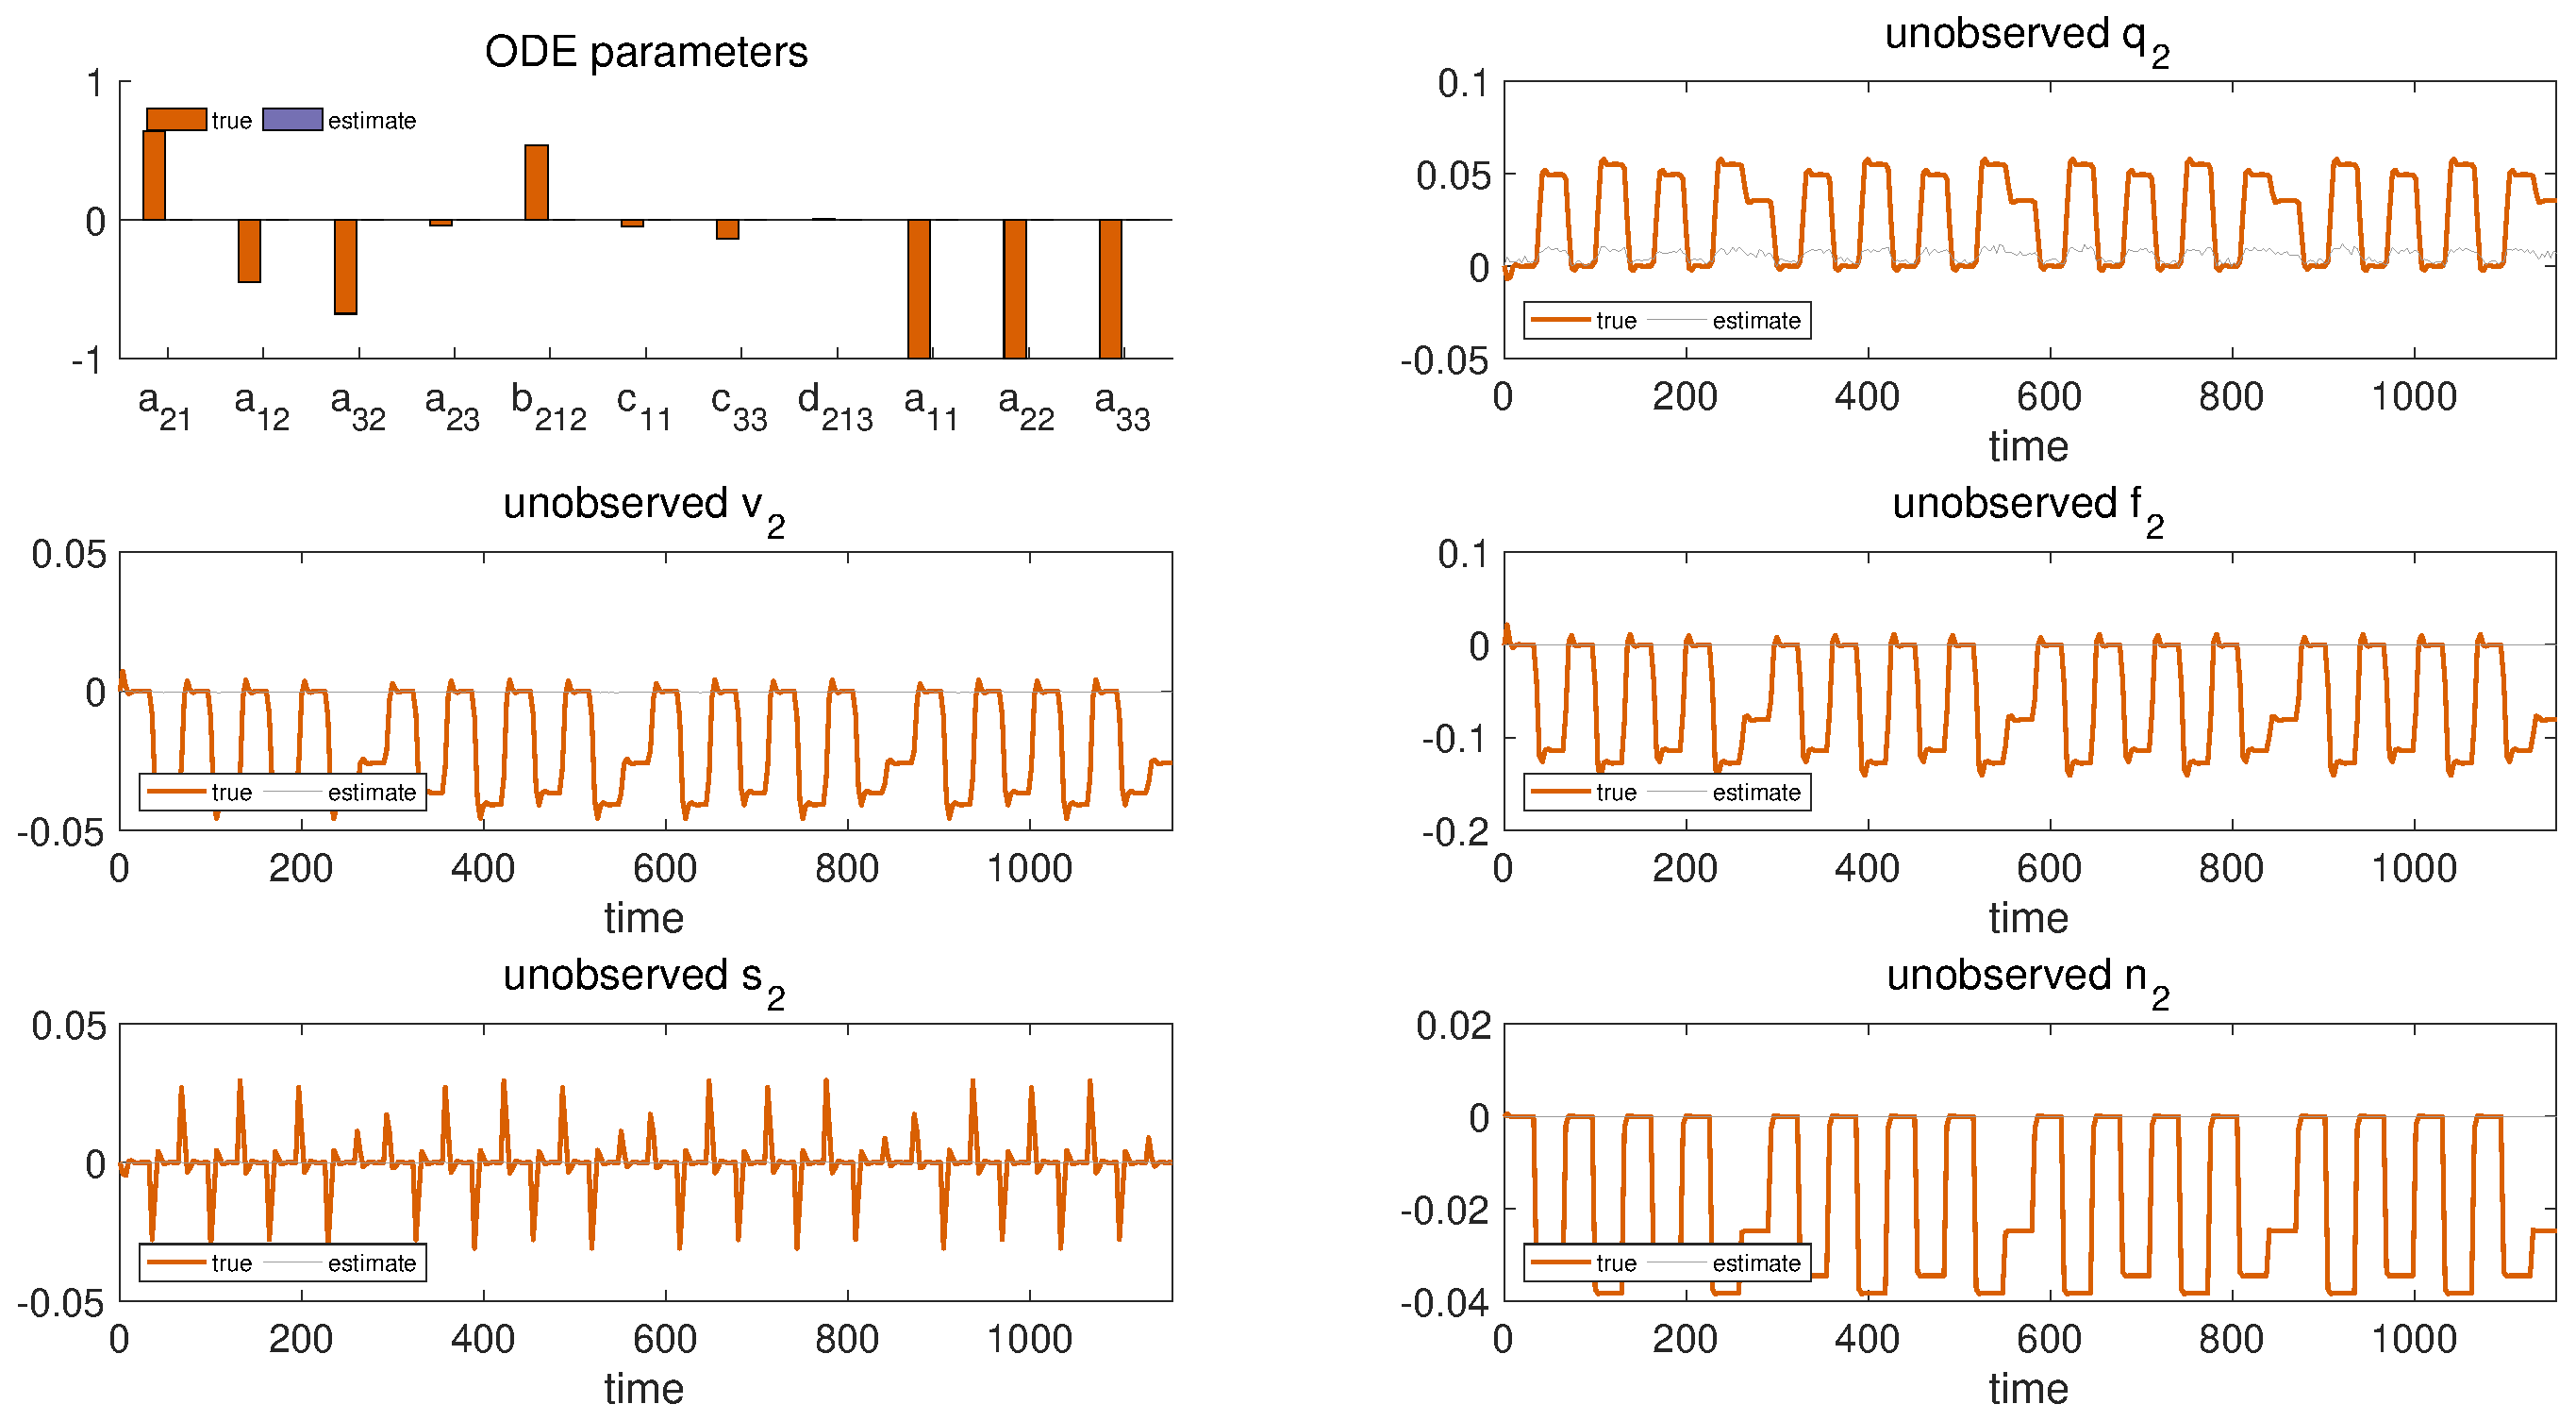
\includegraphics [width=4in]{VGM_for_dynamic_causal_modeling_03.eps}

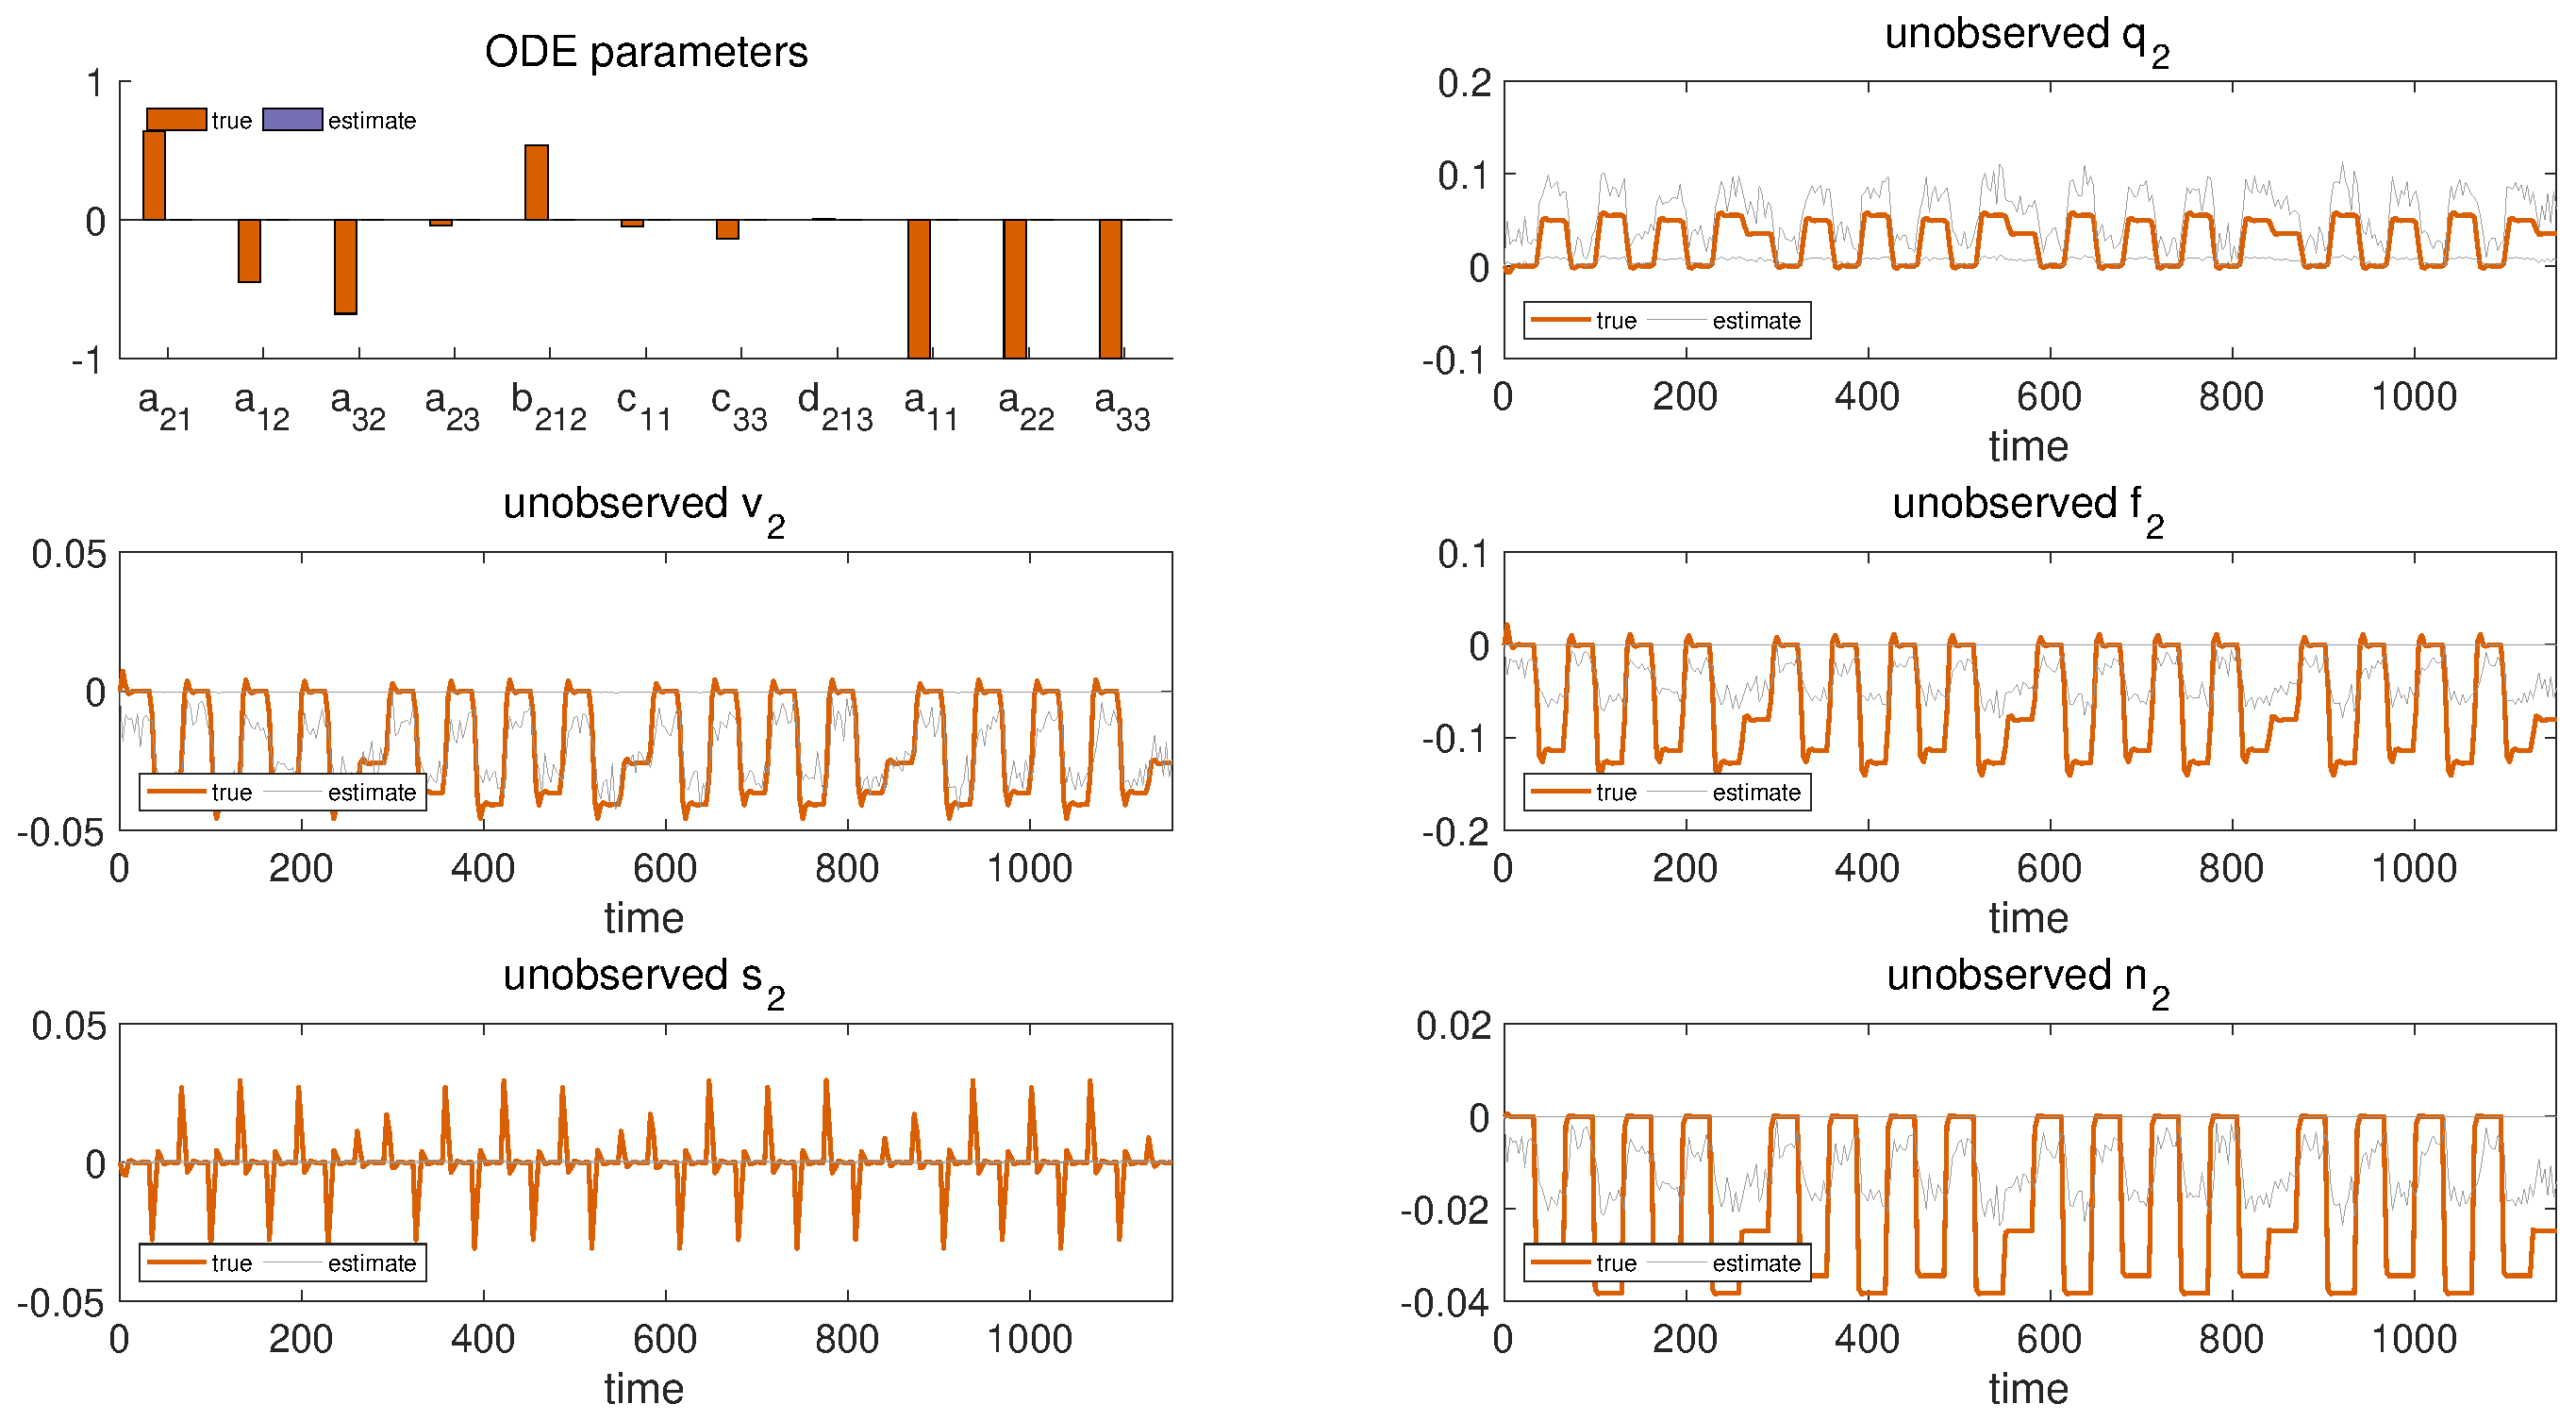
\includegraphics [width=4in]{VGM_for_dynamic_causal_modeling_04.eps}

\includegraphics [width=4in]{VGM_for_dynamic_causal_modeling_05.eps}
\begin{verbatim}
end
\end{verbatim}


\subsection*{}



\subsection*{}



\subsection*{\textbf{Numerical Integration with Estimated ODE Parameters}}

\begin{par}

\end{par} \vspace{1em}
\begin{par}
See whether we actually fit the BOLD responses well. Curves are shown in black.
\end{par} \vspace{1em}
\begin{verbatim}
simulation2 = simulation_old; simulation2.ode_param = ode_param.proxy.mean';
[simulation2,obs_to_state_relation] = simulate_state_dynamics_dcm(simulation2,symbols,ode,time,...
    plot_settings,state.ext_input,'no plot');
state.proxy.num_int = simulation2.state;
\end{verbatim}
\begin{par}

\end{par} \vspace{1em}
\begin{par}
Final Results
\end{par} \vspace{1em}
\begin{verbatim}
plot_results(fig_handle,state.proxy,simulation,ode_param.proxy.mean,plot_handle,symbols,...
    plot_settings,'final',simulation2.bold_response_true,simulation.odes,candidate_odes);
\end{verbatim}

\includegraphics [width=4in]{VGM_for_dynamic_causal_modeling_06.eps}

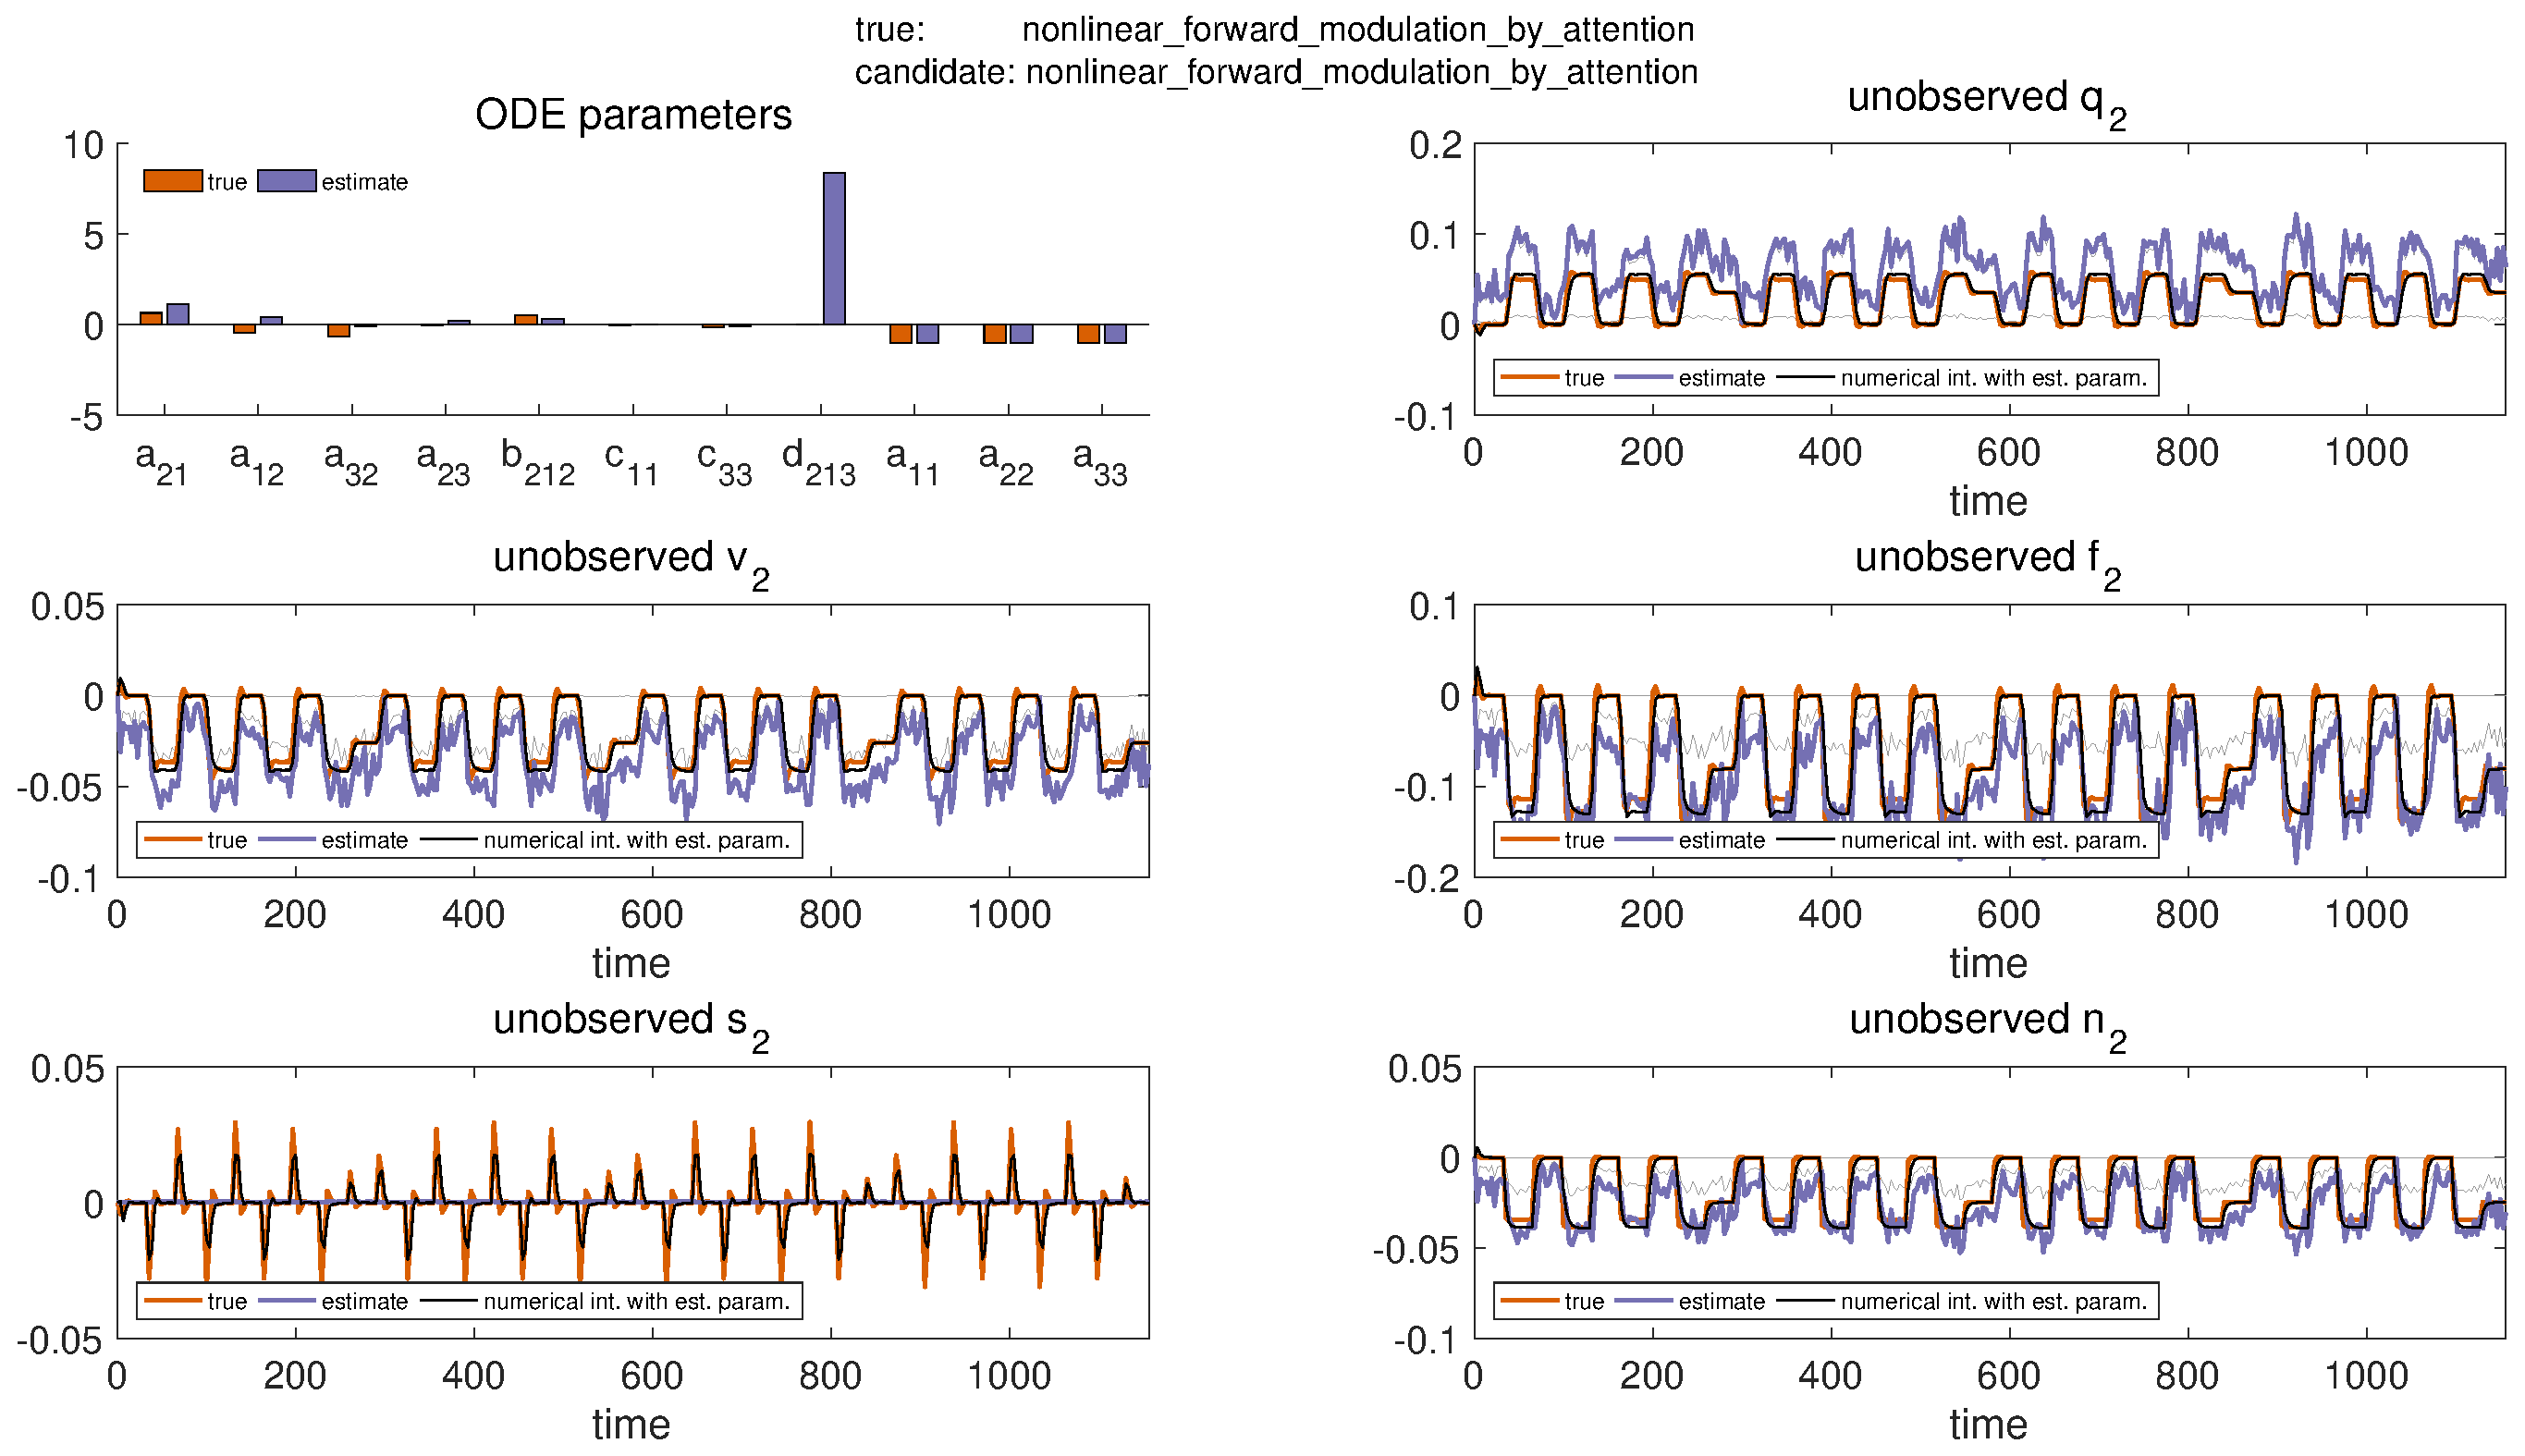
\includegraphics [width=4in]{VGM_for_dynamic_causal_modeling_07.eps}


\subsection*{Time Taken}

\begin{verbatim}
disp(['time taken: ' num2str(toc) ' seconds'])
\end{verbatim}

        \color{lightgray} \begin{verbatim}time taken: 25.8028 seconds
\end{verbatim} \color{black}
    

\subsection*{References}

\begin{par}
*Gorbach, N.S. , Bauer, S. *and Buhmann, J.M., Scalable Variational Inference for Dynamical Systems. 2017a. Neural Information Processing Systems (NIPS). Link to NIPS paper \begin{verbatim}here\end{verbatim} and arxiv paper \begin{verbatim}here\end{verbatim}.
\end{par} \vspace{1em}
\begin{par}
\textbf{Bauer, S. , Gorbach, N.S.} and Buhmann, J.M., Efficient and Flexible Inference for Stochastic Differential Equations. 2017b. Neural Information Processing Systems (NIPS). Link to NIPS paper \begin{verbatim}here\end{verbatim}.
\end{par} \vspace{1em}
\begin{par}
Wenk, P., Gotovos, A., Bauer, S., Gorbach, N.S., Krause, A. and Buhmann, J.M., Fast Gaussian Process Based Gradient Matching for Parameters Identification in Systems of Nonlinear ODEs. 2018. In submission to Conference on Uncertainty in Artificial Intelligence (UAI). Link to arxiv paper \begin{verbatim}here\end{verbatim}.
\end{par} \vspace{1em}
\begin{par}
Calderhead, B., Girolami, M. and Lawrence. N.D., 2002. Accelerating Bayesian inference over nonlinear differential equation models. In Advances in Neural Information Processing Systems (NIPS) . 22.
\end{par} \vspace{1em}
\begin{par}
The authors in \textbf{bold font} have contributed equally to their respective papers.
\end{par} \vspace{1em}



\end{document}
    
